\section{Method}
%------------------------------------------------------------------------------------------
% Outline

% Overview
This section will initially recount all equipment and software used in the project. Following that, a detailed description of the robots design and sensors, followed by an overview of the major software: ROS2, SLAM Toolbox and Navigation2. Finally the testing environments and testing scenarios will be detailed together with a description of the simulated and real-world systems in the respective sections.

%======================================================
% Components

% Component list
The complete list of all components used in the project:
\begin{enumerate}
    \item 2D LIDAR: \href{https://www.mouser.se/ProductDetail/426-DFR0315}{Slamtec RPLiDAR A1}, see\:\cite{slamtec_rplidar_2016} for sensor specifications.
    \item 6-DOF IMU: \href{https://www.mouser.se/ProductDetail/426-SEN0142}{InvenSense MPU6050}, see\:\cite{invensense_mpu-6000_2013} for sensor specifications.
    \begin{itemize}
        \item 3-DOF MEMS gyroscope, see\:\cite{invensense_mpu-6000_2013} for sensor specifications.
        \item 3-DOF MEMS accelerometer, see\:\cite{invensense_mpu-6000_2013} for sensor specifications.
    \end{itemize}
    \item $2 \times \text{Wheel encoders}$\footnote{No wheel encoder specifications were available.}: N/A. The wheel encoders are integrated into the motorized wheels, see\:\ref{enum:motorized_wheels} Motorized wheels.
    \item \label{enum:motorized_wheels} $2 \times \text{Motorized wheels}$: \href{https://www.amazon.se/dp/B07WP3XDLC?psc=1&ref=ppx_yo2ov_dt_b_product_details}{Garosa Magnetic Gear Motor Wheel DC 12V}
    \item $2 \times \text{Spherical wheels}$: \href{https://www.mouser.se/ProductDetail/485-3948}{Metal Caster Bearing Wheel}
    \item Central control unit: \href{https://www.electrokit.com/en/raspberry-pi-4-model-b/8gb}{Raspberry Pi 4 Model B/8GB}
    \item Motor control unit: \href{https://store.arduino.cc/products/arduino-nano}{Arduino Nano}
    \item Motor driver: \href{https://www.electrokit.com/en/motordrivare-l298-dubbel-h-brygga-5-35v-2a}{Motor driver L298 dual H-bridge 5-35V 2A}
    \item Data storage: \href{https://www.inet.se/produkt/5304540/samsung-microsd-evo-plus-64gb}{Samsung MicroSD EVO Plus 64GB}
    \item Power source: \href{https://hobbyking.com/en_us/turnigy-battery-3000mah-3s-20c-lipo-pack-xt-60.html?___store=en_us}{Turnigy 3000mAh 3S 20C Lipo Pack w/XT-60}
    \item Charger: \href{https://www.amazon.se/-/en/gp/product/B087G199LH/ref=ewc_pr_img_1?smid=ADG7ML0RBF414&psc=1}{Lipo Battery Balanced Charger}
    \item Buck converter: \href{https://www.electrokit.com/en/dc-dc-omvandlare-step-down-1.25-35v-5a}{DC-DC converter step-down 1.25-35V 5A}
    \item Fuse holder: \href{https://www.conrad.se/sv/p/tru-components-tc-9070404-sakringsinsats-passar-till-flatsakring-standard-30-a-32-v-dc-1-st-2267601.html}{TRU COMPONENTS TC-9070404 30 A 32 V/DC}
    \item Fuse: \href{https://www.conrad.se/sv/p/eska-340127-340-127-standardflatsakring-10-a-rod-1-st-535104.html}{ESKA 340127 340.127 10A}
    \item Toggle switch: \href{https://www.electrokit.com/en/vippomkopplare-med-skylt-1-pol-on-off}{SparkFun Toggle switch}
    \item Jumper cables
    \item 22 AWG wires
    \item Chassis: 3D printed, see Fig.\:\ref{fig:robot_chassis}.
\end{enumerate}
A full list of all the components can also be found on the \href{https://github.com/MobiBotInnovate}{Github}\footnote{https://github.com/MobiBotInnovate\label{foot1}} page for the project.

%======================================================
% Specs

\begin{comment}

% LIDAR specs
\begin{table}
    \centering
    \begin{tabular}{|c|c|c|} \hline
         \textbf{Parameter}     & \textbf{Unit}                 & \textbf{Typical}          \\ \hline
         Distance Range         & Meter ($\text{m}$)            & $0.15-6$                  \\
         Distance Resolution    & Millimeter ($\text{mm}$)      & $1\%$ of the distance     \\ \hline
         Angular Range          & Degree ($\degree$)            & $0-360$                   \\
         Angular Resolution     & Degree ($\degree$)            & $1$                       \\ \hline
         Noise Performance      & N/A                           & Not specified             \\ \hline
    \end{tabular}
    \caption{RPLiDAR A1 specifications\:\cite{slamtec_rplidar_2016}.}
    \label{tab:lidar_specs}
\end{table}

% IMU Gyroscope specs
\begin{table}
    \centering
    \resizebox{\columnwidth}{!}{\noindent\begin{tabular}{|c|c|c|c|c|c|} \hline
        \textbf{Parameter}                                      & \textbf{Conditions}                               & \textbf{Unit}                                     & \textbf{Min}      & \textbf{Typical}      & \textbf{max}      \\ \hline
        Full-Scale Range                                        & $\text{FS\_SEL} = 0$                              & $\degree / \text{s}$                              &                   & $\pm 250$             &                   \\
                                                                & $\text{FS\_SEL} = 1$                              & $\degree / \text{s}$                              &                   & $\pm 500$             &                   \\
                                                                & $\text{FS\_SEL} = 2$                              & $\degree / \text{s}$                              &                   & $\pm 1000$            &                   \\
                                                                & $\text{FS\_SEL} = 3$                              & $\degree / \text{s}$                              &                   & $\pm 2000$            &                   \\ \hline
        Sensitivity Scale Factor                                & $\text{FS\_SEL} = 0$                              & $\frac{\text{LSB}}{\degree / \text{s}}$           &                   & $131$                 &                   \\
                                                                & $\text{FS\_SEL} = 1$                              & $\frac{\text{LSB}}{\degree / \text{s}}$           &                   & $65.5$                &                   \\
                                                                & $\text{FS\_SEL} = 2$                              & $\frac{\text{LSB}}{\degree / \text{s}}$           &                   & $32.8$                &                   \\
                                                                & $\text{FS\_SEL} = 3$                              & $\frac{\text{LSB}}{\degree / \text{s}}$           &                   & $16.4$                &                   \\ \hline
        Sensitivity Scale Factor Tolerance                      & $25\degree\text{C}$                               & $\%$                                              & $-3$              &                       & $+3$              \\
        Sensitivity Scale Factor Variation Over Temperature     &                                                   & $\%$                                              &                   & $\pm 2$               &                   \\ 
        Nonlinearity                                            & Best Fit Straight Line; $25\degree\text{C}$       & $\%$                                              &                   & $0.2$                 &                   \\
        Cross-Axis Sensitivity                                  &                                                   & $\%$                                              &                   & $\pm 2 $              &                   \\ \hline
        \textbf{Noise Performance}                              & $\text{FS\_SEL} = 0$                              &                                                   &                   &                       &                   \\
        Total RMS Noise                                         & $\text{DLPFCFG} = 2 \: (100\:\text{Hz})$          & $\degree / \text{s-rms}$                          &                   & $0.05$                &                   \\
        Low-frequency RMS noise                                 & Bandwidth $1\:\text{Hz}$ to $10\:\text{Hz}$       & $\degree / \text{s-rms}$                          &                   & $0.033$               &                   \\
        Rate Noise Spectral Density                             & $@10\:\text{Hz}$                                  & $\frac{\degree / \text{s}}{\sqrt{\text{Hz}}}$     &                   & $0.005$               &                   \\ \hline
    \end{tabular}}
    \caption{MPU6050 MEMS gyroscope specifications\:\cite{invensense_mpu-6000_2013}.}
    \label{tab:imu_gyro_specs}
\end{table}

% IMU Accelerometer specs
\begin{table}
    \centering
    \resizebox{\columnwidth}{!}{\noindent\begin{tabular}{|c|c|c|c|} \hline
        \textbf{Parameter}                      & \textbf{Conditions}                                                           & \textbf{Unit}                                 & \textbf{Typical}      \\ \hline
        Full-Scale Range                        & $\text{AFS\_SEL} = 0$                                                         & $\text{g}$                                    & $\pm 2$               \\
                                                & $\text{AFS\_SEL} = 1$                                                         & $\text{g}$                                    & $\pm 4$               \\
                                                & $\text{AFS\_SEL} = 2$                                                         & $\text{g}$                                    & $\pm 8$               \\
                                                & $\text{AFS\_SEL} = 3$                                                         & $\text{g}$                                    & $\pm 16$              \\ \hline
        Sensitivity Scale Factor                & $\text{AFS\_SEL} = 0$                                                         & $\frac{\text{LSB}}{\text{g}}$                 & $16384$               \\
                                                & $\text{AFS\_SEL} = 1$                                                         & $\frac{\text{LSB}}{\text{g}}$                 & $8192$                \\
                                                & $\text{AFS\_SEL} = 2$                                                         & $\frac{\text{LSB}}{\text{g}}$                 & $4096$                \\
                                                & $\text{AFS\_SEL} = 3$                                                         & $\frac{\text{LSB}}{\text{g}}$                 & $2048$                \\ \hline
        Sensitivity Change vs. Temperature      & $\text{AFS\_SEL} = 0$, $-40 \degree \text{C}$ to $+85 \degree \text{C}$       & $\frac{\%}{\degree\text{C}}$                  & $\pm 0.02$            \\ 
        Nonlinearity                            & Best Fit Straight Line                                                        & $\%$                                          & $0.5$                 \\
        Cross-Axis Sensitivity                  &                                                                               & $\%$                                          & $\pm 2 $              \\ \hline
        \textbf{Noise Performance}              &                                                                               &                                               &                       \\
        Power Spectral Density                  & $@10\:\text{Hz}$, $\text{AFS\_SEL} = 0$ \& $\text{ODR} = 1\:\text{kHz}$       & $\frac{ \mu \text{g}}{\sqrt{\text{Hz}}}$      & $400$                 \\ \hline
    \end{tabular}}
    \caption{MPU6050 MEMS accelerometer specifications\:\cite{invensense_mpu-6000_2013}.}
    \label{tab:imu_acc_specs}
\end{table}

% Wheel encoder specs
\begin{table}
    \centering
    \begin{tabular}{|c|c|c|} \hline
         \textbf{Parameter}     & \textbf{Unit}                 & \textbf{Typical}          \\ \hline
         Range                  & N/A                           & Not specified             \\ \hline
         Noise Performance      & N/A                           & Not specified             \\ \hline
    \end{tabular}
    \caption{Wheel encoder specifications. No wheel encoder specifications were available.}
    \label{tab:encoder_specs}
\end{table}

\end{comment}

%======================================================
% Software

% Software list
Software specifications and toolboxes used:
\begin{enumerate}
    \item 3D Design Tool: \href{https://www.autodesk.com/products/fusion-360/personal}{Autodesk Fusion 360} version 2.0.18950 x86\_64
    \item Operating system:
    \begin{itemize}
        \item Simulation: Ubuntu 22.04.4 LTS, with \href{https://docs.ros.org/en/humble/index.html}{ROS2}\:\cite{macenski_impact_2023}\cite{macenski_robot_2022} running on top of it.
        \item Real-world:
        \begin{itemize}
            \item PC: Ubuntu 22.04.4 LTS, with \href{https://docs.ros.org/en/humble/index.html}{ROS2}\:\cite{macenski_impact_2023}\cite{macenski_robot_2022} running on top of it.
            \item Robot: 
            \begin{itemize}
                \item Raspberry Pi: Ubuntu Server 22.04.4 LTS, with \href{https://docs.ros.org/en/humble/index.html}{ROS2}\:\cite{macenski_impact_2023}\cite{macenski_robot_2022} running on top of it.
                \item Arduino Nano: N/A. The Arduino Nano is only running compiled code, see\:\ref{enum:programming_language} Programming language.
            \end{itemize}
        \end{itemize}
    \end{itemize}
    \item \label{enum:programming_language}Programming language:
    \begin{itemize}
        \item Arduino Nano: \href{https://www.arduino.cc/reference/en/}{Arduino programming language} version 1.8.19
        \item Other: Python3 version 3.10.6
    \end{itemize}
    \item Robot communication and interaction: 
    \begin{itemize}
        \item Simulation: \href{https://docs.ros.org/en/humble/index.html}{ROS2}\:\cite{macenski_impact_2023}\cite{macenski_robot_2022} version 3.5.1
        \item Real-world:
        \begin{itemize}
            \item PC: \href{https://docs.ros.org/en/humble/index.html}{ROS2}\:\cite{macenski_impact_2023}\cite{macenski_robot_2022} version 3.5.1
            \item Robot:
            \begin{itemize}
                \item Raspberry Pi: \href{https://docs.ros.org/en/humble/index.html}{ROS2}\:\cite{macenski_impact_2023}\cite{macenski_robot_2022} version 3.5.1
            \end{itemize}
        \end{itemize}
    \end{itemize}
    \item ROS-visualization tool:
    \begin{itemize}
        \item Simulation: \href{https://turtlebot.github.io/turtlebot4-user-manual/software/rviz.html}{Rviz2} humble version 11.2.12 
        \item Real-world:
        \begin{itemize}
            \item PC: \href{https://turtlebot.github.io/turtlebot4-user-manual/software/rviz.html}{Rviz2} humble version 11.2.12 
        \end{itemize}
    \end{itemize}
    \item SLAM:
    \begin{itemize}
        \item Simulation: \href{https://wiki.ros.org/slam_toolbox}{SLAM Toolbox}\:\cite{macenski_slam_2021}\cite{macenski_use_2019} humble version 2.6.8
        \item Real-world: 
        \begin{itemize}
            \item PC: \href{https://wiki.ros.org/slam_toolbox}{SLAM Toolbox}\:\cite{macenski_slam_2021}\cite{macenski_use_2019} humble version 2.6.8
        \end{itemize}
    \end{itemize}
    \item Navigation and path planning:
    \begin{itemize}
        \item Simulation: \href{https://navigation.ros.org/tutorials/docs/navigation2_with_slam.html}{Navigation2}\:\cite{macenski_desks_2023}\cite{macenski_open-source_2024}\cite{macenski_regulated_2023}\cite{merzlyakov_comparison_2021}\cite{macenski_marathon_2020} humble version 1.1.15 
        \item Real-world:
        \begin{itemize}
            \item PC: \href{https://navigation.ros.org/tutorials/docs/navigation2_with_slam.html}{Navigation2}\:\cite{macenski_desks_2023}\cite{macenski_open-source_2024}\cite{macenski_regulated_2023}\cite{merzlyakov_comparison_2021}\cite{macenski_marathon_2020} humble version 1.1.15
        \end{itemize}
    \end{itemize}
    \item Simulation tool: \href{https://gazebosim.org/home}{Gazebo 11}
\end{enumerate}

% MIT and Github
All code developed is open source under the MIT License and available on \href{https://github.com/MobiBotInnovate}{Github}\footref{foot1}.

%------------------------------------------------------------------------------------------
% Design

\subsection{Design}

% Raspberry Pi and Arduino Nano
The Arduino Nano was chosen for motor control because it supported available motor device drivers, as well as Raspberry Pi lacking analog to digital conversion (ADC) pins. Since the Raspberry Pi is more powerful, and can run Linux (Ubuntu) and ROS2, it performed all remaining software tasks. Note that this does not include sensor fusion, SLAM and path planning which were run on an external PC in real-world testing, see Method\:\ref{subsection:real_world}.
% Robot chassis
The chassis of the circular differential drive robot can be seen in Fig.\:\ref{fig:robot_chassis} and consisted of two circular plates with a radius of $100\:\text{mm}$, the complete design files can be found on \href{https://github.com/MobiBotInnovate}{Github}\footref{foot1}. 
\begin{figure}
    \centering
	\begin{subfigure}[t]{0.49\columnwidth}
		\centering
		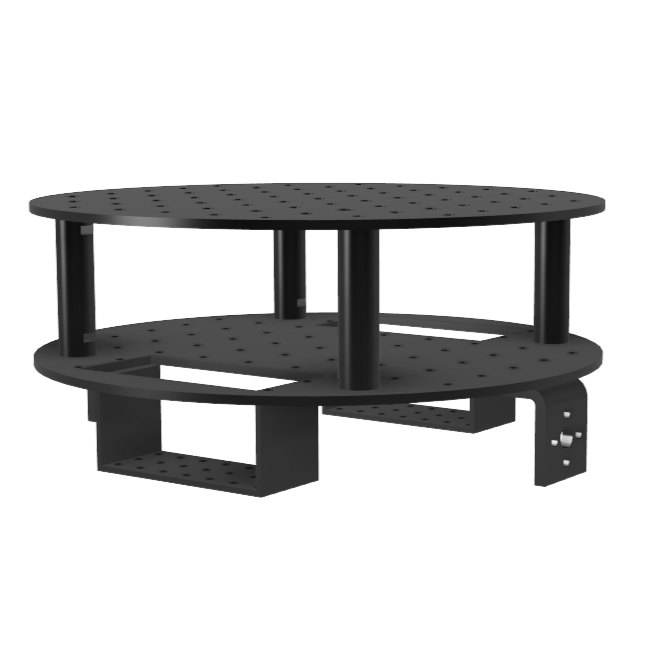
\includegraphics[width=\textwidth]{images/model_top.png}
		\caption{Side view of the robot chassis with both base and top plate visible.}
        \label{fig:top_chassis}
	\end{subfigure}
    \hfill
	\begin{subfigure}[t]{0.49\columnwidth}
		\centering
		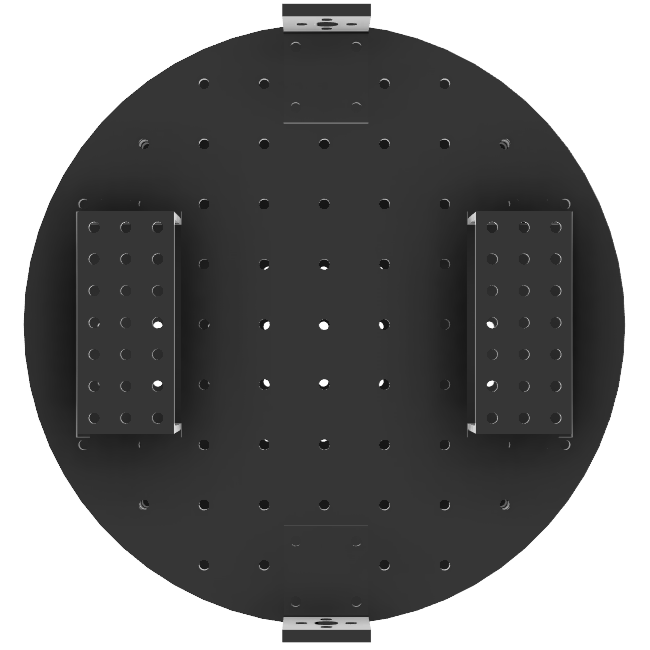
\includegraphics[width=\textwidth]{images/model_bot.png}
		\caption{Bottom view of robot chassis, only base plate visible.}
        \label{fig:bottom_chassis}
	\end{subfigure}
	\caption{The 3D printed robot chassis.}
    \label{fig:robot_chassis}
\end{figure}
% Wiring diagram
A wiring diagram for all the electrical components can be seen in Fig.\:\ref{fig:wiringD}.
\begin{figure}
    \centering
    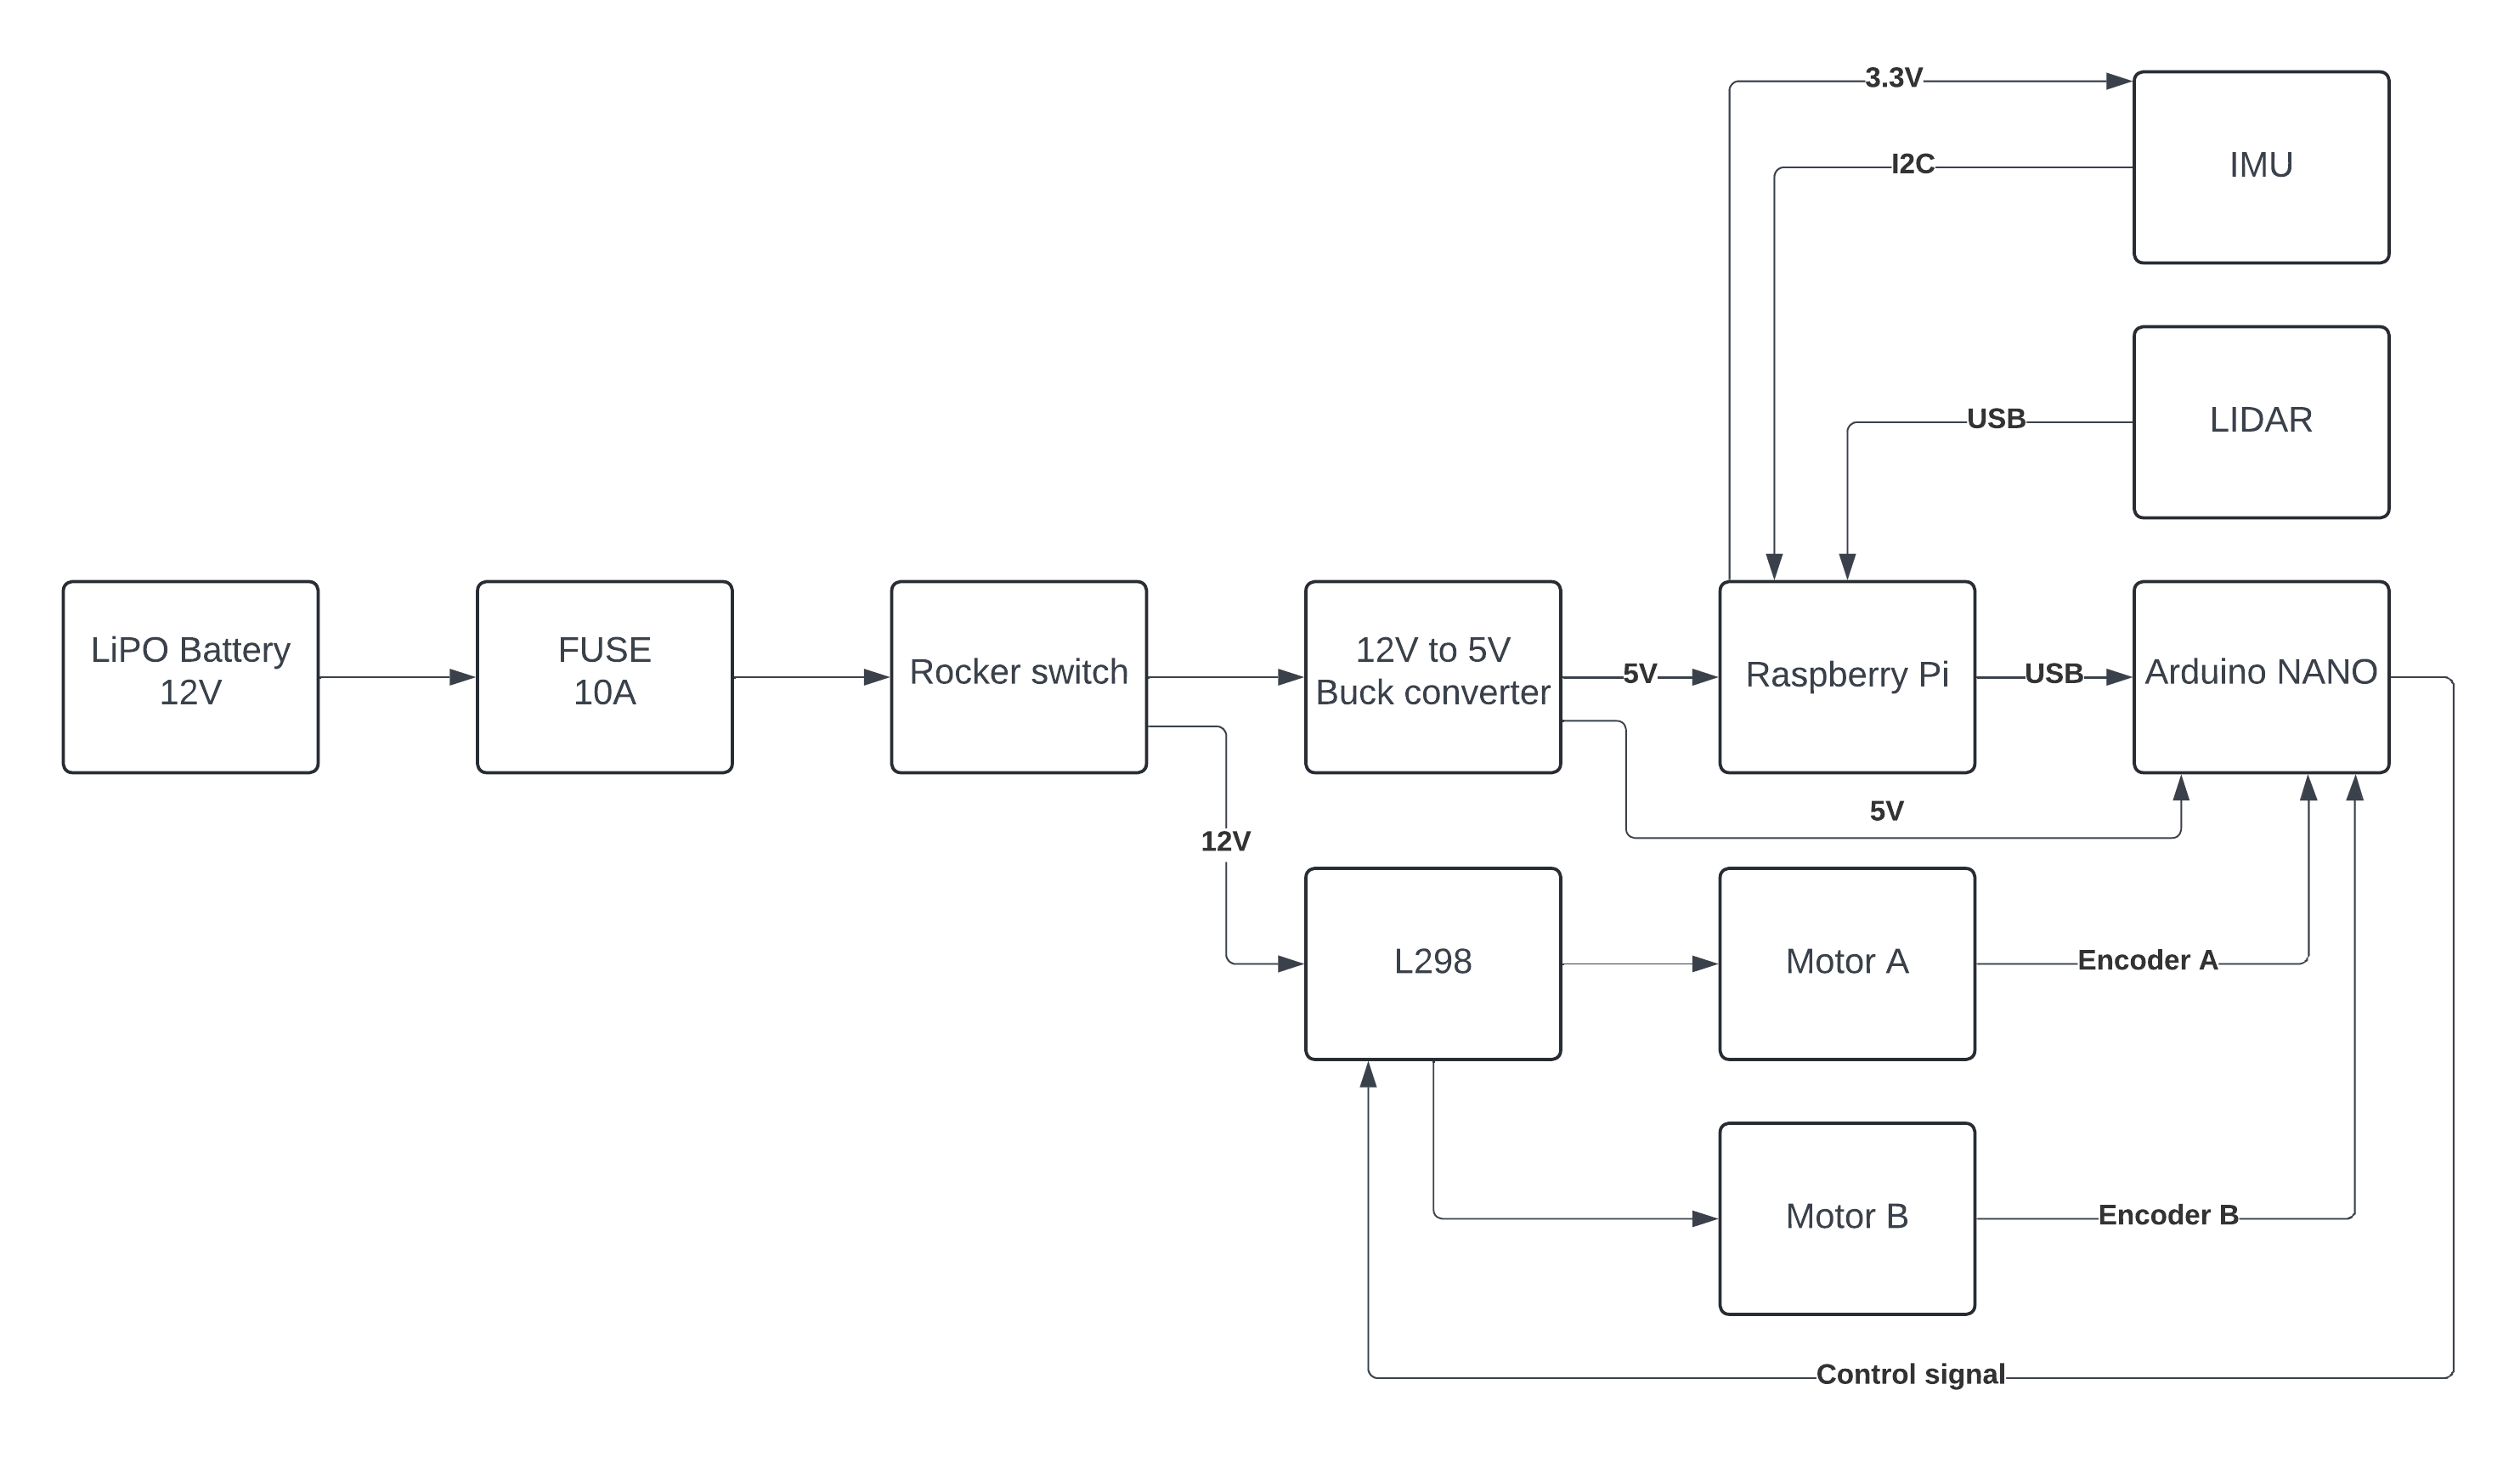
\includegraphics[width=\columnwidth]{images/wiringD.png}
    \caption{Wiring diagram for all electrical components.}
    \label{fig:wiringD}
\end{figure}
% Locations of parts on chassis
The LIDAR and the power source were attached to the top plate of the robot chassis, see Fig.\:\ref{fig:constructed_robot_top_plate}. Mounted on the upper side of the base plate were: the Raspberry Pi, Arduino Nano, IMU, toggle switch, buck converter and fuses, as can be seen in Fig.\:\ref{fig:constructed_robot_top}, with motor driver installed on the bottom side of the base plate, see Fig.\:\ref{fig:constructed_robot_bot}. The motorized wheels were attached to the middle of the base plate, with one spherical wheel attached in the front and one in the back to balance it, see Fig.\:\ref{fig:constructed_robot_bot}. 
% 4 wheel reason
Given that the axle of the motorized wheels runs along the middle of the robot, a single stabilizing wheel proved insufficient, necessitating an additional stabilizing wheel to prevent tipping, especially during acceleration.

% Final real world robot
The finalized robot which was used for real-world testing can be seen in Fig.\:\ref{fig:constructed_robot}.
\begin{figure}
    \centering
    \begin{subfigure}[t]{0.32\columnwidth}
        \centering
        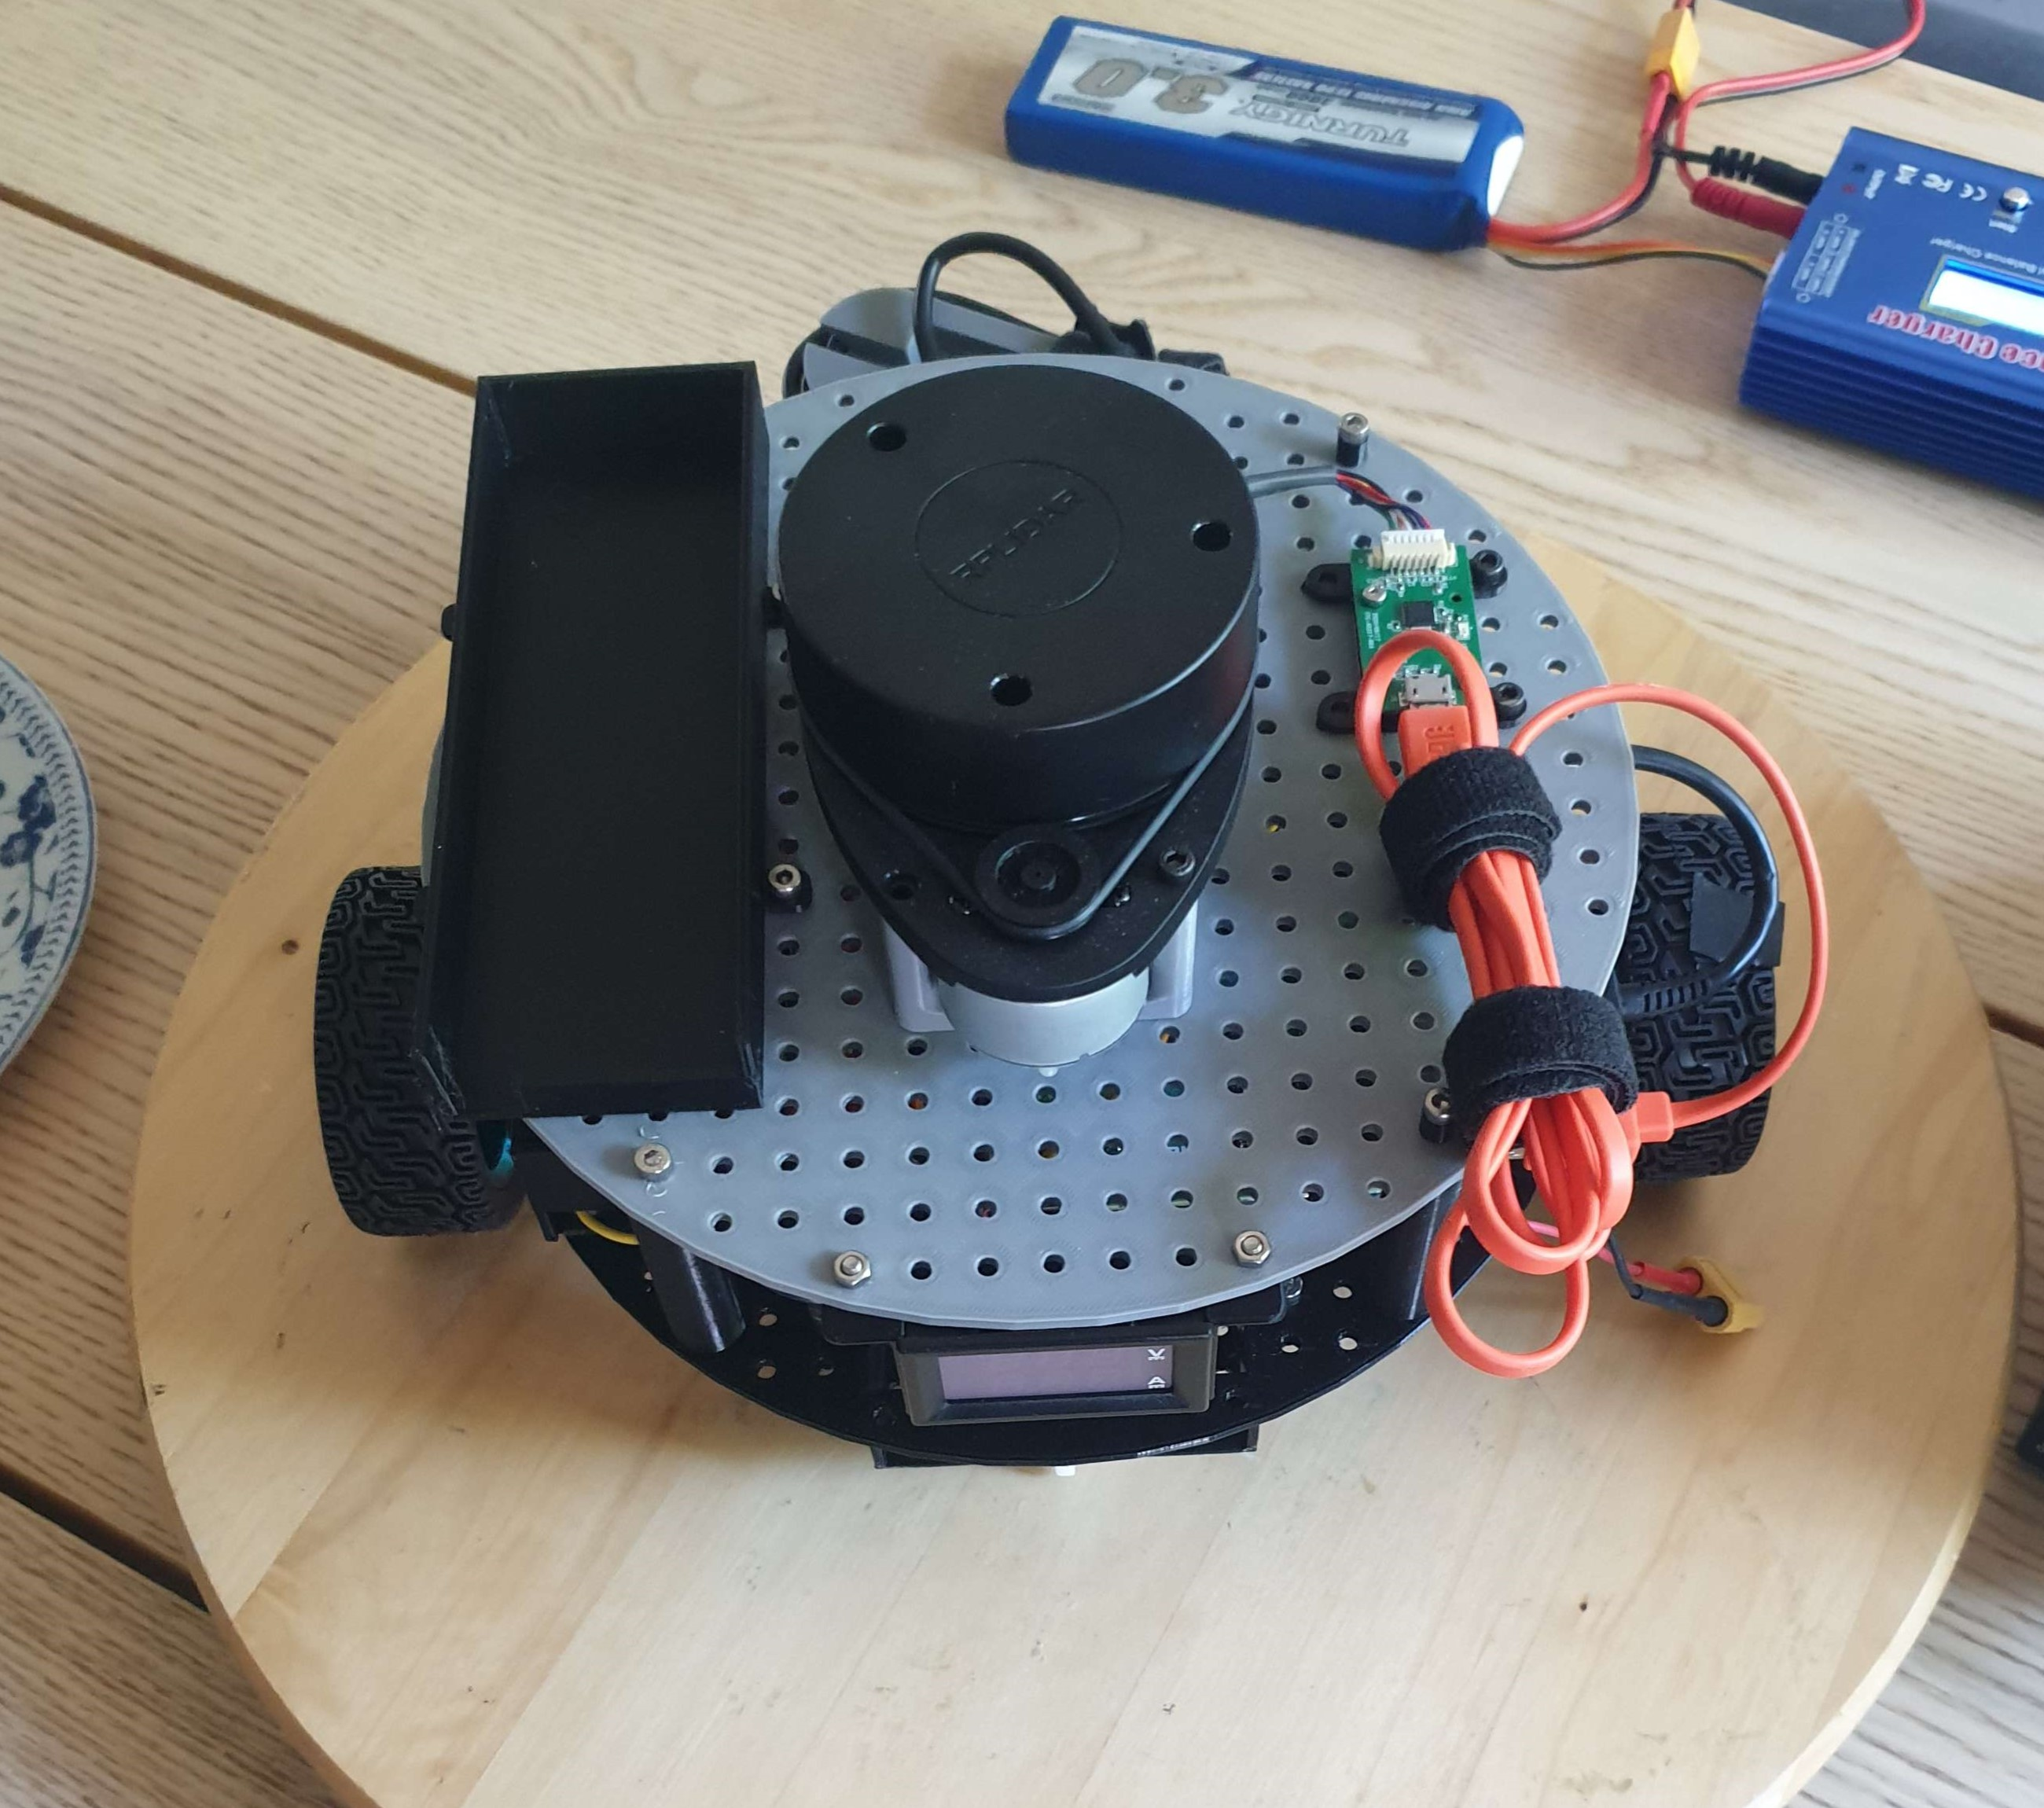
\includegraphics[width=\textwidth]{images/real_robot_top_plate.jpg}
        \caption{Top view of the constructed robot, with top plate attached.}
        \label{fig:constructed_robot_top_plate}
    \end{subfigure}
    \hfill
	\begin{subfigure}[t]{0.32\columnwidth}
		\centering
		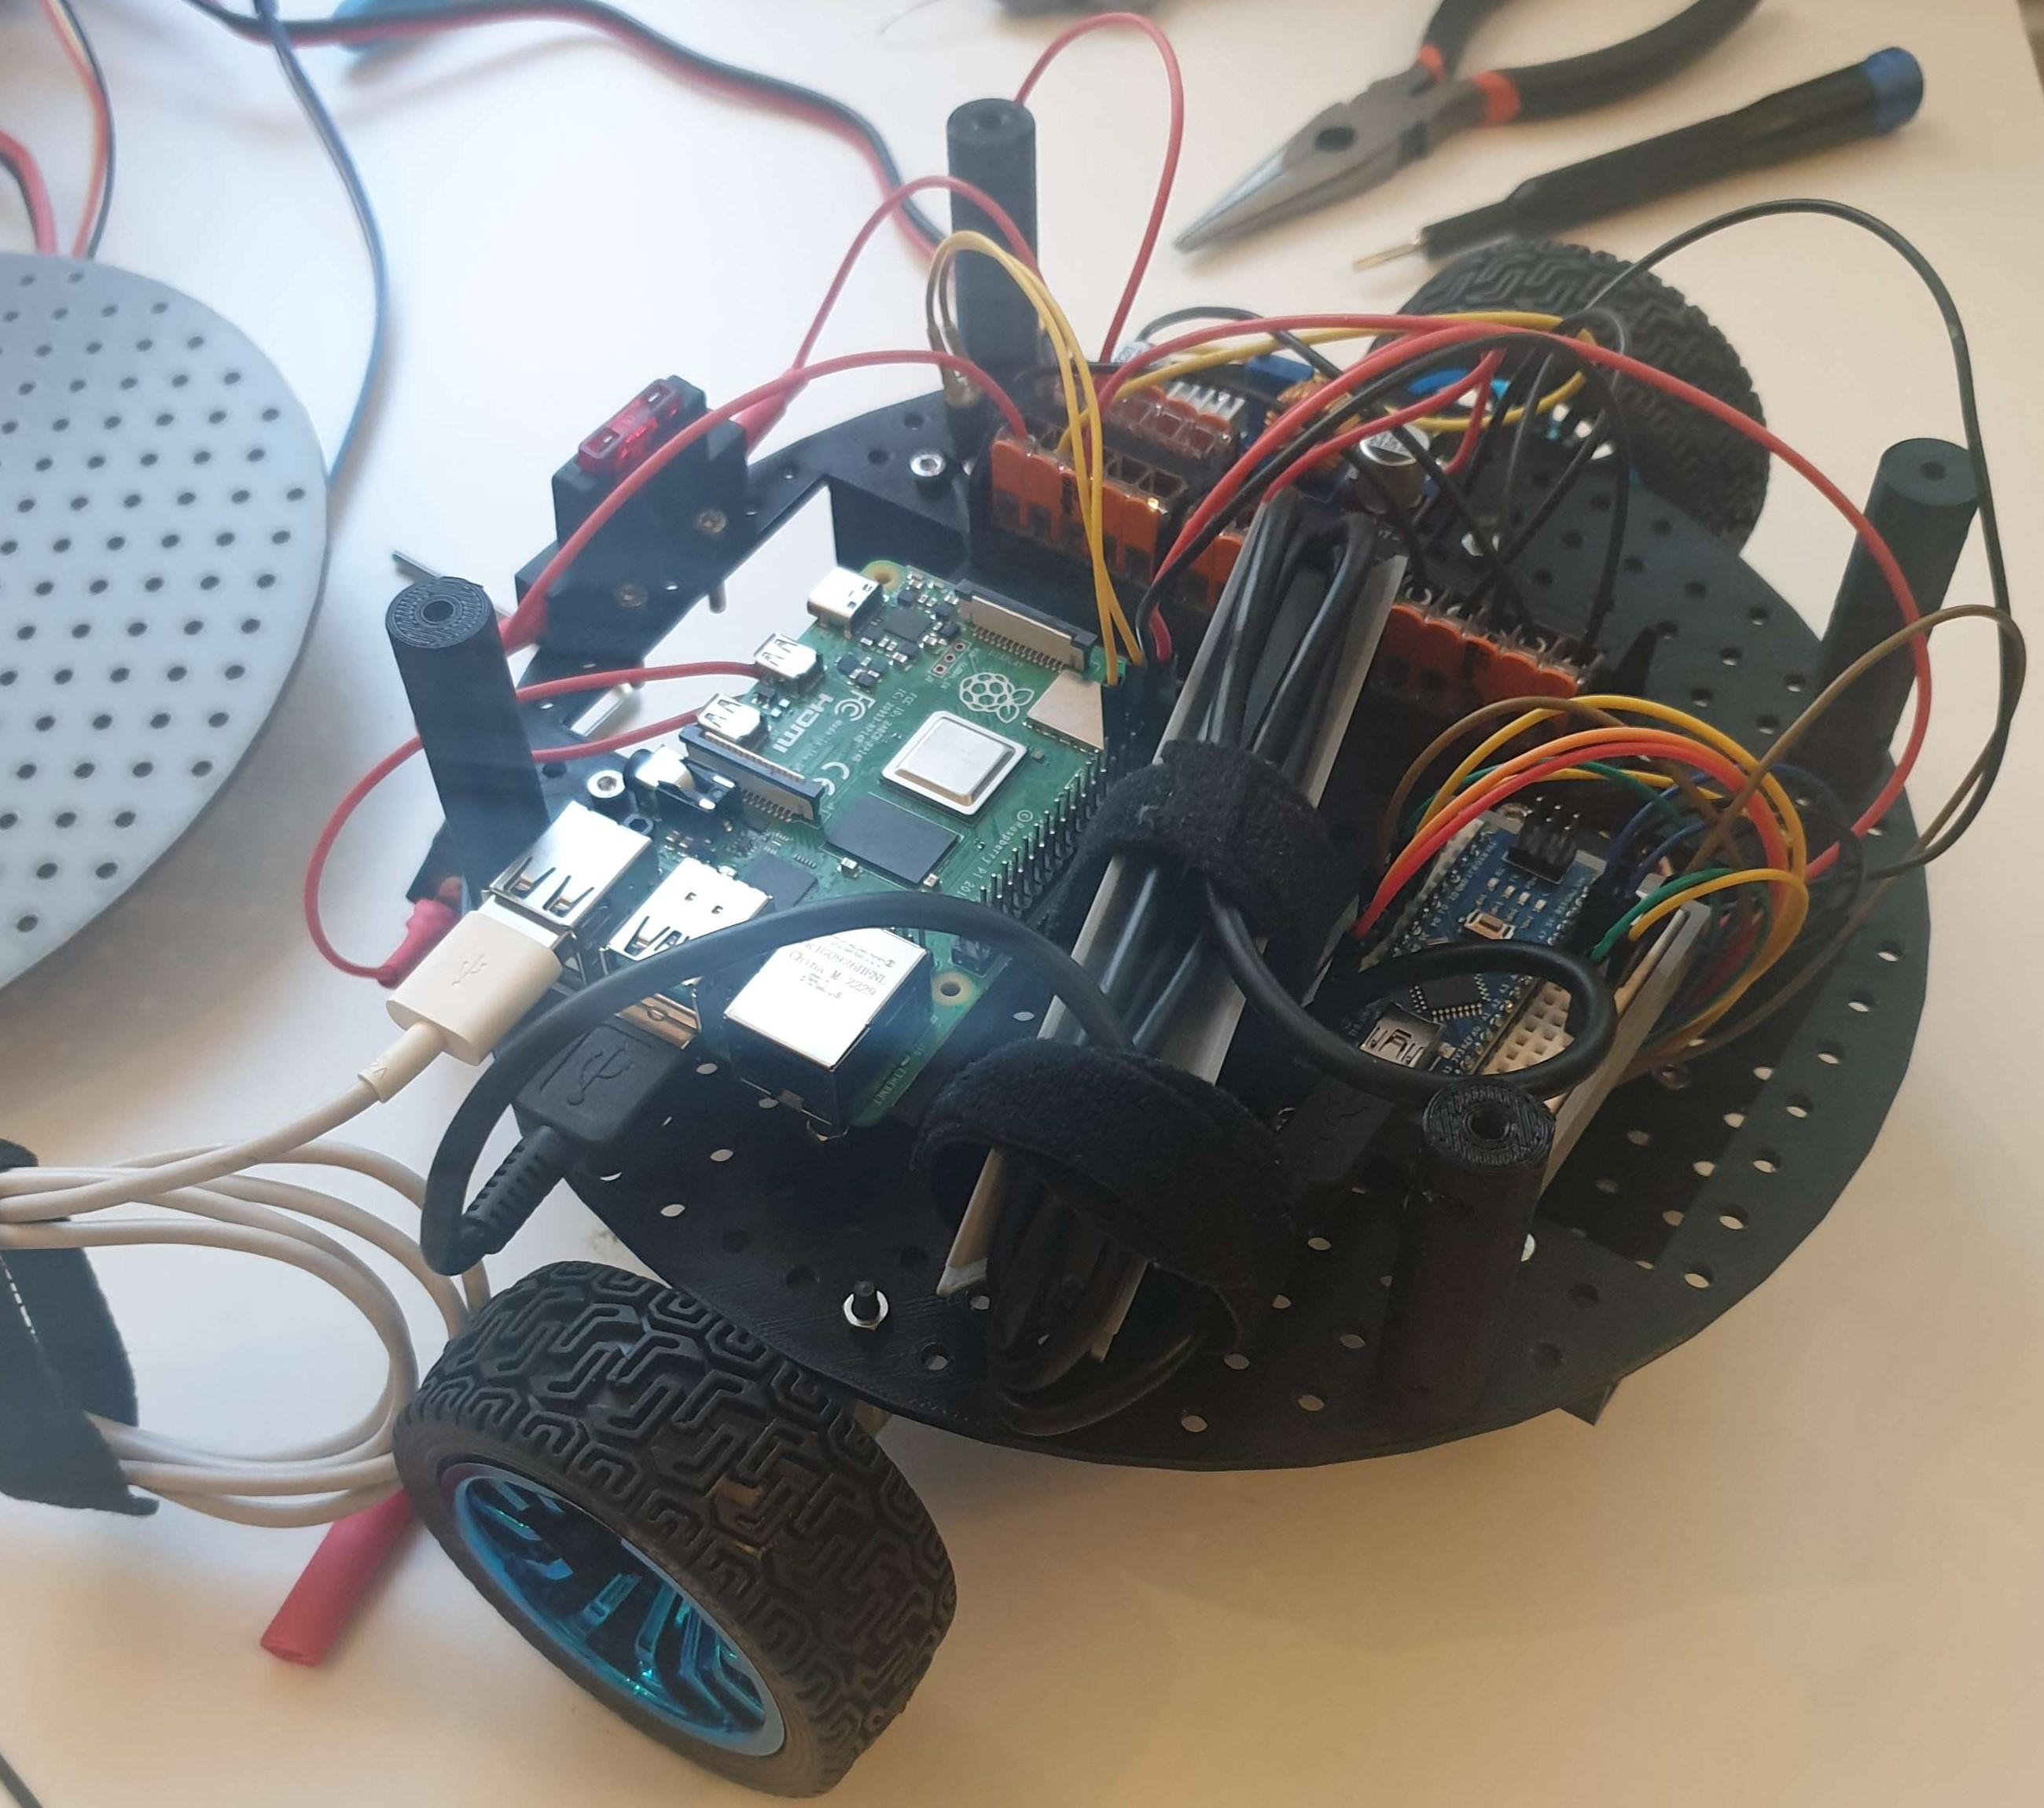
\includegraphics[width=\textwidth]{images/real_robot_top.jpg}
		\caption{Top view of the constructed robot, with top plate removed for clarity of component locations.}
        \label{fig:constructed_robot_top}
	\end{subfigure}
    \hfill
	\begin{subfigure}[t]{0.32\columnwidth}
		\centering
		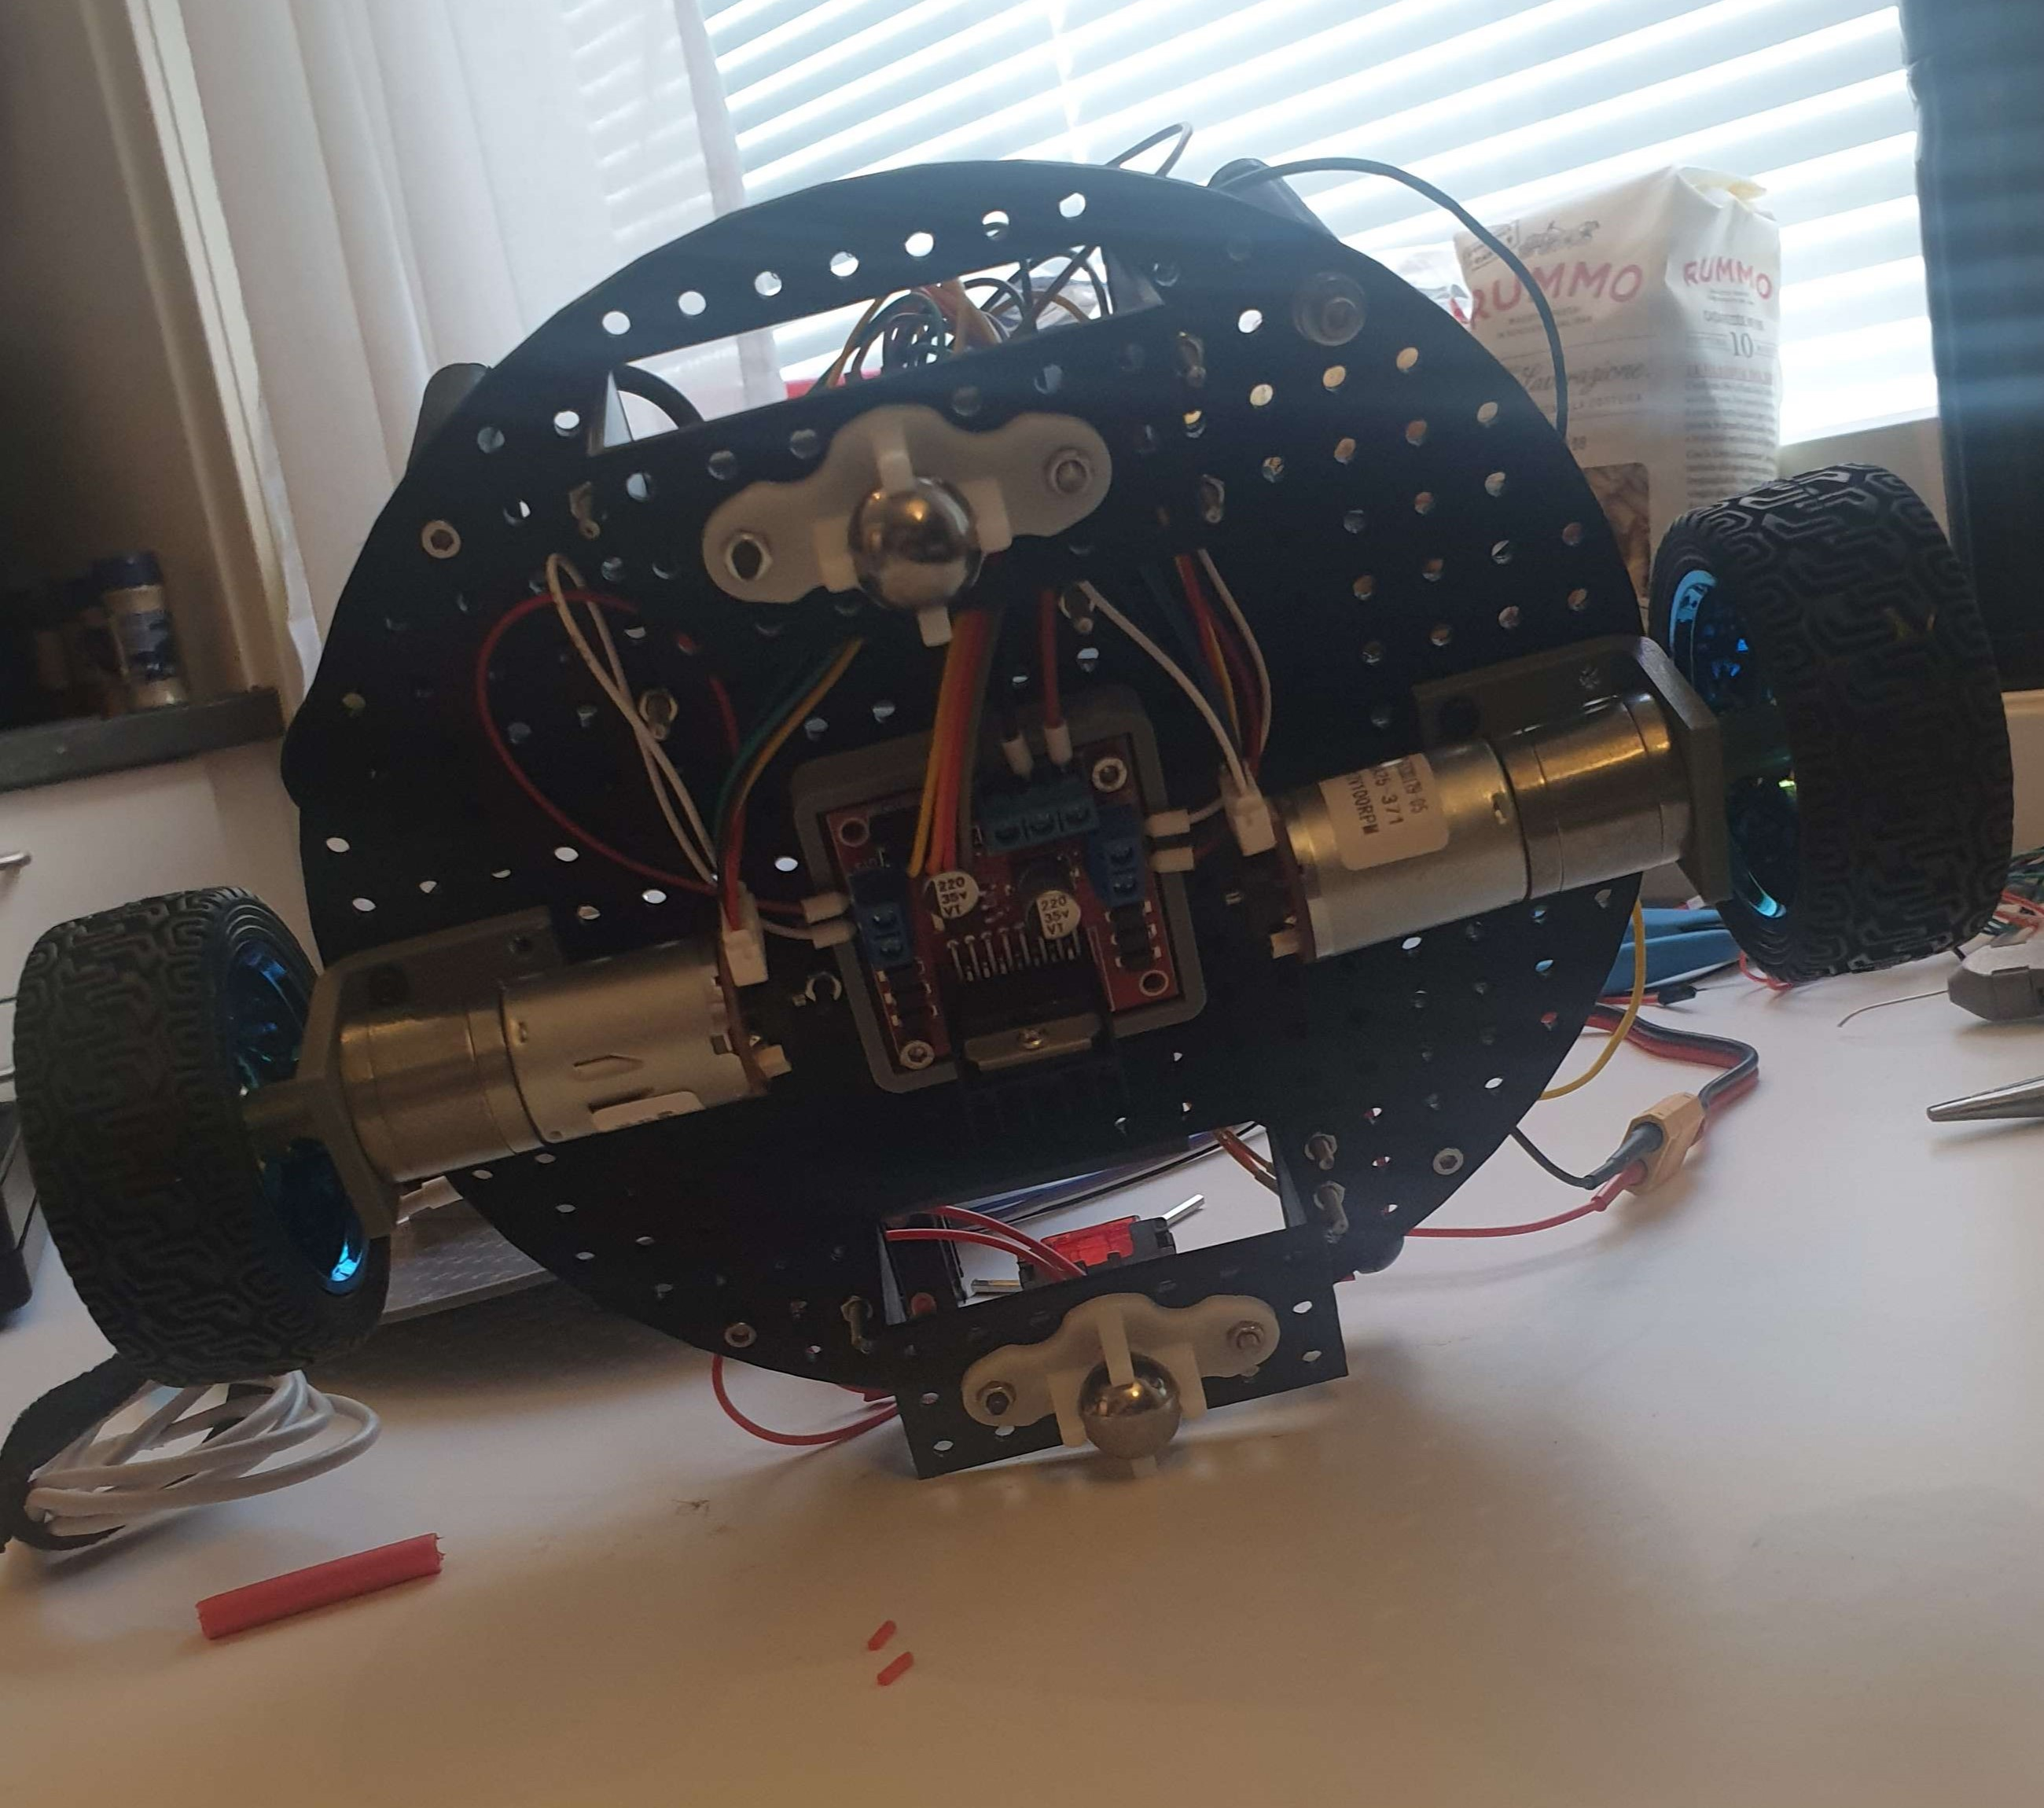
\includegraphics[width=\textwidth]{images/real_robot_bot.jpg}
		\caption{Bottom view of the constructed robot.}
        \label{fig:constructed_robot_bot}
	\end{subfigure}
    \caption{The finalized robot used for real-world testing.}
    \label{fig:constructed_robot}
\end{figure}

%------------------------------------------------------------------------------------------
% Sensors

\subsection{Sensors}

% Purpose
This project used two wheel encoders and a \href{https://www.mouser.se/ProductDetail/426-SEN0142}{6-DOF IMU}, consisting of a 3-DOF MEMS (microelectromechanical system) gyroscope and accelerometer\:\cite{invensense_mpu-6000_2013}, for obtaining odometry information as suggested by the Introduction\:\ref{section:intro}. A \href{https://www.mouser.se/ProductDetail/426-DFR0315}{2D LIDAR} was used for measuring the surrounding, given its compatibility with the toolboxes used and the criteria established, see Introduction\:\ref{section:intro}.

% BAISC FUNCTIONALITY OF SENSORS WHICH ONLY CONCERNS ELA400
% THIS FILE IS ELA400 SPECIFIC, CONTAINING SENSOR FUNCTIONALITY INFORMATION WHICH IS NOT NECESSARY FOR ELA408
%------------------------------------------------------------------------------------------

% !!! LEAVE EMPTY FOR ELA408 REPORT !!!

%------------------------------------------------------------------------------------------

%------------------------------------------------------------------------------------------

% ROS2

\subsection{ROS2}

% Overview
ROS2 contributes to easy development of robotic systems and applications, it offers middleware, algorithms and developer tools\:\cite{macenski_robot_2022}. 
% Purpose
The integration of ROS2 is crucial for easy and quick development as well as its critical purpose in the system. Handling communication, interaction between different parts of the system, and being compatible with the toolboxes used\:\cite{macenski_impact_2023}\cite{macenski_robot_2022}.

% TOOLBOX INFORMATION WHICH ONLY CONCERNS ELA408
% THIS FILE IS ELA408 SPECIFIC, CONTAINING TOOLBOX INFORMATION WHICH IS NOT NECESSARY FOR ELA400
%------------------------------------------------------------------------------------------

% Overview
ROS2 was developed to provide modular and distributed systems, allowing much of the work to be reused and easily adapted to new and similar applications, facilitating collaboration and cooperation\:\cite{macenski_robot_2022}. It has real time capabilities and works on embedded systems as well as in diverse network conditions and environments\:\cite{macenski_robot_2022}.
% Features
% Sensor fusion
Among all of the the features offered by ROS2, one of them is sensor fusion, using either an extended Kalman filter (EKF) or an unscented Kalman filter (UKF)\:\cite{macenski_desks_2023}. 
% Localization
It also offers an AMCL (adaptive Monte Carlo localization) package for localization\:\cite{macenski_desks_2023}. 
% Utility functions
Additionally, ROS2 offers a number of utility functions to improve safety by giving commands, regulating and validating the robotic system and its navigation\:\cite{macenski_desks_2023}. Included in these are collision monitoring which overrides the navigation planner in case of emergencies, and lifecycle manger which ensures that the system starts up and shuts down in a safe and deterministic manner\:\cite{macenski_desks_2023}. 
% More info
For additional information about features offered by ROS2, see\:\cite{macenski_desks_2023}, and for a deeper understanding of ROS2, see\:\cite{macenski_robot_2022}.

%------------------------------------------------------------------------------------------


%------------------------------------------------------------------------------------------
\begin{comment}
    
\end{comment}
%------------------------------------------------------------------------------------------

% Default and changed parameters
The ROS2 parameters which were changed from their default value are shown in Fig.\:\ref{tab:ros2_params_changed}, parameters which are not listed had their default value.
\begin{table}
    \centering
    \begin{tabular}{|c|c|} \hline
         \textbf{Parameter}         & \textbf{Value}    \\ \hline
         Sensor fusion              & EKF               \\ \hline
    \end{tabular}
    \caption{ROS2 parameters which were changed from their default value.}
    \label{tab:ros2_params_changed}
\end{table}
EKF was used for sensor fusion since it provided the best results.

%------------------------------------------------------------------------------------------
% SLAM

\subsection{SLAM Toolbox}

% Purpose
The SLAM tool used in this project is an open source toolbox called SLAM Toolbox, which is built on top of OpenKarto SLAM\:\cite{macenski_slam_2021}\cite{macenski_desks_2023}\cite{macenski_use_2019}.
% World model
SLAM Toolbox uses elastic pose-graph representation for localization and mapping\:\cite{macenski_use_2019}, which can be converted to a 2D probabilistic occupancy grid map\:\cite{macenski_slam_2021}. 
% Scan matching, loop closure, link matching, scan correlation
It offers scan matching (which uses a correlation grid), loop closing, link matching algorithm and scan correlation\:\cite{macenski_slam_2021}.

% TOOLBOX INFORMATION WHICH ONLY CONCERNS ELA408
% THIS FILE IS ELA408 SPECIFIC, CONTAINING TOOLBOX INFORMATION WHICH IS NOT NECESSARY FOR ELA400
%------------------------------------------------------------------------------------------

% Boasted features
SLAM Toolbox boasts a number of impressive features compared to its competitors, including\:\cite{macenski_slam_2021}:
\begin{itemize}
    \item Being able to map areas as large as $9000\:\text{m}^2$
    \item Serialize (save) and deserialize (load) map, allowing for continued expanding of a previous map
    \item Being able to merge multiple maps using kinematic map merging
    \item Being able to perform synchronous mapping, asynchronous mapping or pure localization
    \item Faster measurement matching, better optimization and more (see\:\cite{macenski_slam_2021})
\end{itemize}
% Lifelong mapping
It offers has a functionality called lifelong mapping which not only allows SLAM to continue refining the map and update it, but also remove redundant and outdated data by the help of a heuristic\:\cite{macenski_use_2019}. 
% KD-Tree
On top of that it also makes use of k-dimensional trees (KD-Tree) to perform search matching (nearest neighbor search matching) for localization of the robot position\:\cite{macenski_slam_2021}.
% Parameters etc
A subset of the parameter options offered by SLAM Toolbox are outlined in Table.\:\ref{tab:slam_toolbox_params}\:\cite{macenski_slam_2021}\cite{macenski_use_2019}.
\begin{table}
    \centering
    \resizebox{\columnwidth}{!}{\noindent\begin{tabular}{|c|c|} \hline
         \textbf{Parameter}                                         & \textbf{Options}                                      \\ \hline
         Nonlinear solver                                           & Ceres solver                                          \\
                                                                    & SPA solver                                            \\
                                                                    & g2o solver                                            \\ \hline
         Linear solver used by Ceres                                & sparse Cholesky factorization                         \\
                                                                    & Schur complement                                      \\
                                                                    & Schur complement and iterative solver                 \\
                                                                    & CGNR (conjugate gradient normal residual)             \\ \hline
         Preconditioner  to use with linear solver                  & Identity (none)                                       \\
                                                                    & Jacobi                                                \\
                                                                    & Schur complement Jacobi                               \\ \hline
         Ceres trust region strategy                                & Levenberg-Marquardt algorithm                         \\
                                                                    & Dogleg algorithm                                      \\ \hline
         Dogleg strategy to use if the trust strategy is Dogleg     & Traditional Dogleg                                    \\
                                                                    & Subspace Dogleg                                       \\ \hline
         Loss function to reject outliers                           & None                                                  \\
                                                                    & Huber loss                                            \\
                                                                    & Cauchy loss                                           \\ \hline
        KD-Tree distance metric                                     & Manhattan distance functor                            \\ 
                                                                    & Squared Euclidean distance functor                    \\
                                                                    & Squared Euclidean (L2) distance functor               \\
                                                                    & SO2 distance functor                                  \\
                                                                    & SO3 distance functor (uses L2\_Simple)                \\ \hline
    \end{tabular}}
    \caption{A subset of the parameter options offered by SLAM Toolbox\:\cite{macenski_slam_2021}\cite{macenski_use_2019}.}
    \label{tab:slam_toolbox_params}
\end{table}

%------------------------------------------------------------------------------------------


%------------------------------------------------------------------------------------------
\begin{comment}
    %The occupancy grid map has default scale of $1\:\text{grid coordinate} = 1\:\text{pixel} = 0.05\:\text{meters}$\:\cite{macenski_slam_2021}\cite{macenski_use_2019}.    
\end{comment}
%------------------------------------------------------------------------------------------

% Default and changed parameters
The default parameters of SLAM Toolbox has been shown to perform the best in normal situations\:\cite{macenski_slam_2021}\cite{macenski_use_2019}, minimal alterations were therefor attempted. All parameters which were changed from their default value are shown in Table.\:\ref{tab:slam_toolbox_params_changed}.
\begin{table}
    \centering
    \begin{tabular}{|c|c|} \hline
         \textbf{Parameter}         & \textbf{Value}    \\ \hline
         Laser\_range               & 6.0               \\ \hline
         Barycentering              & False             \\ \hline
         map\_update\_interval      & 1.0               \\ \hline
         scan\_buffer\_size         & 100               \\ \hline
         stack\_size\_to\_use       & 90000000          \\ \hline
    \end{tabular}
    \caption{SLAM Toolbox parameters which were changed from their default.}
    \label{tab:slam_toolbox_params_changed}
\end{table}
Laser\_range was changed because of the LIDAR used. Barycentering was set to False and scan pose was thus used instead of barycentering since it made the mapping more accurate. The remaining parameters were found during testing to provide the best performance.

% SLAM Toolbox Flowchart
The complete functionality of SLAM Toolbox can be seen in Fig.\:\ref{fig:slam_toolbox}.
\begin{figure*}
    \centering
    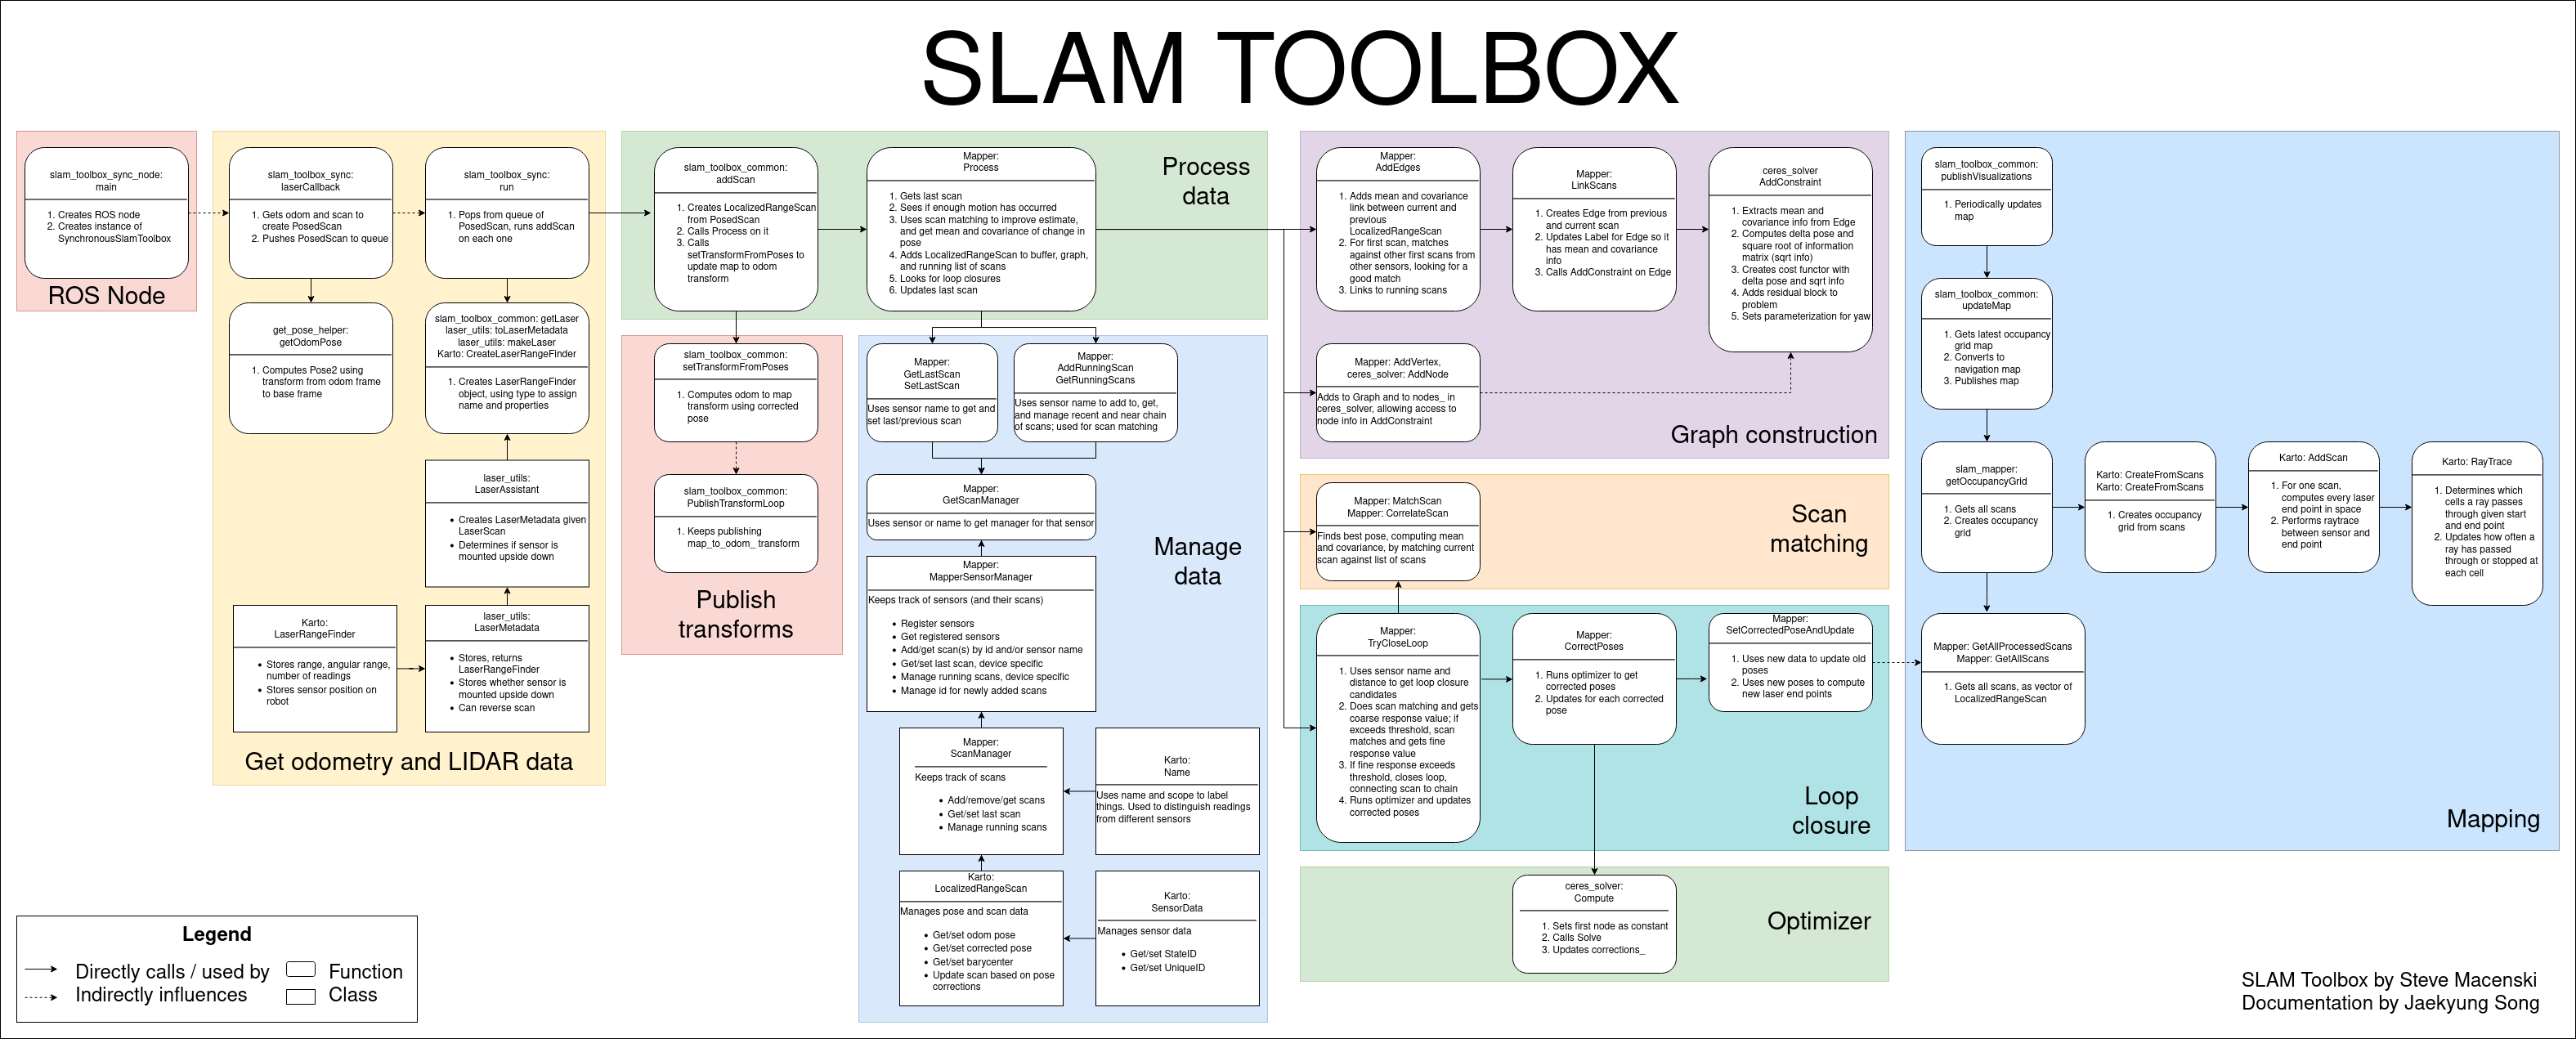
\includegraphics[width=\textwidth]{images/slam_toolbox_sync.png}
    \caption{SLAM Toolbox flowchart showing the functionality of the toolbox. Courtesy of Steven Macenski (creator)\:\cite{macenski_slam_2021}\cite{macenski_use_2019}.}
    \label{fig:slam_toolbox}
\end{figure*}

%------------------------------------------------------------------------------------------
% Navigation

\subsection{Navigation2}

% Purpose
This project used the optimized open source toolbox Navigation2 (Nav2), for proficient robot navigation and path planning\:\cite{macenski_desks_2023}\cite{macenski_open-source_2024}\cite{macenski_regulated_2023}\cite{merzlyakov_comparison_2021}\cite{macenski_marathon_2020}.
% Global, local and recovery
Nav2 performs three tasks: planning (global path planning), control (local trajectory tracking) and recovery, orchestrated by a configurable behavior tree\:\cite{macenski_marathon_2020}. The three tasks are nodes in the behavior tree with the navigator as the root, all of them sharing a costmap model of the environment\:\cite{macenski_marathon_2020}.

% TOOLBOX INFORMATION WHICH ONLY CONCERNS ELA408
% THIS FILE IS ELA408 SPECIFIC, CONTAINING TOOLBOX INFORMATION WHICH IS NOT NECESSARY FOR ELA400
%------------------------------------------------------------------------------------------

% Outline
The design of Nav2 makes it very configurable and expandable, it also works for a multitude of robot types in a wide range of applications and environments\:\cite{macenski_marathon_2020}. It has also been shown to be safe, deterministic, reliable and robust in dynamic settings even during extended time frames\:\cite{macenski_marathon_2020}. 

% Global path planning
% Smac planner (templated A*)
Smac planner is the standard global path planning system used by Nav2\:\cite{macenski_open-source_2024}. It uses a templated A* which performs search, and it is templated by node planner templates NodeT which implements the different planner-specifics\:\cite{macenski_open-source_2024}. With this, NodeT can select different templates which results in different planners and characteristics\:\cite{macenski_open-source_2024}. All the planners thus share the same A* algorithm but the cost function and neighborhood selection policies are decoupled\:\cite{macenski_open-source_2024}. This is further clarified when inspecting the node planners which contain two things\:\cite{macenski_open-source_2024}:
\begin{itemize}
    \item Node state: which includes things like collision state, visited status, queued status and accumulated cost of the node in the graph
    \item Planner-specific: which includes how traversal costs should be computed, heuristics and expansion characteristics
\end{itemize}
Three different planner templates (NodeT) are offered, these are: cost-aware 2D-A*, cost-aware Hybrid-A* and cost-aware State Lattice\:\cite{macenski_open-source_2024}. Cost-aware means that additional information is encoded in the map and used by the path planner rather than just the common binary info of occupied or free (see costmap in Introduction\:\ref{section:intro})\:\cite{macenski_open-source_2024}.
Finally there is an integration layer which, on the highest level, links the planner with the robot, thus allowing for easy deployment on multiple robotic frameworks\:\cite{macenski_open-source_2024}.
% Smoothing global paths
Nav2 includes three smoothing algorithms to help refine paths produced by the global path planner, these are: Simple Smoother, Constrained Smoother, and Savitzky-Golay Smoother\:\cite{macenski_desks_2023}.
% Additional info
For the complete specifications of Smac planner, see the work by Macenski \textit{et al.}\:\cite{macenski_open-source_2024}.

% Local path planning
% DWB
The default local trajectory tracker used by Navigation2 is DWB, which is an expansion of Dynamic Window Approach (DWA)\:\cite{liu_path_2023}\cite{macenski_desks_2023}. DWB gathers a set of candidate commands, based on its current velocity and dynamic limits, by sub-sampling feasible velocities from a dynamic window, these velocities are projected forward to generate circular arcs (trajectories)\:\cite{macenski_desks_2023}. These arcs are then evaluated using a set of critic functions (which can optimize for different behaviors), and the best is chosen\:\cite{macenski_desks_2023}.
% Additional info
The interested reader is refereed to\:\cite{macenski_desks_2023} for additional information about the local trajectory tracking offered by Nav2.

% Recovery
Recovery behavior is used to prevent complete navigation failure and follows a protocol where initially the actions are conservative and then become more aggressive\:\cite{macenski_marathon_2020}. The actions can be system wide or specific to a certain task like planning and control\:\cite{macenski_marathon_2020}. Example actions include: clearing costmap, waiting and spinning\:\cite{macenski_marathon_2020}.

%------------------------------------------------------------------------------------------


%------------------------------------------------------------------------------------------
\begin{comment}
    , replacing Navigation Function (NavFn)\:\cite{macenski_desks_2023}
    % RPP
    %A local trajectory planner (path tracking) available in Navigation2 is the Regulated Pure Pursuit algorithm (RPP) which is an extension of Adaptive Pure Pursuit (APP)\:\cite{macenski_regulated_2023}. Compared to normal pure pursuit, this variant uses adaptive lookahead distance and takes into account and adapts linear and angular velocity to increase safety and operability, specifically in constrained and partially observable environments\:\cite{macenski_regulated_2023}. It achieves this by incorporating preemptive collision detection, using regulation heuristics and penalizing being close to obstacles as well as taking sharp turns\:\cite{macenski_regulated_2023}. RPP also achieves better efficiency, and thanks to the higher safety it offers, it allows the system to have higher maximum speed while still remaining safe\:\cite{macenski_regulated_2023}.
    % Additional info
    %For a complete understanding of the RPP algorithm see\:\cite{macenski_regulated_2023}.
\end{comment}
%------------------------------------------------------------------------------------------

% Default and changed parameters
All Navigation2 parameters which were altered in this project can be seen in Table.\:\ref{tab:nav2_params_changed}.
\begin{table}
    \centering
    \begin{tabular}{|c|c|} \hline
         \textbf{Parameter}         & \textbf{Value}        \\ \hline
         odom\_topic                & /odometry/filtered    \\ \hline
    \end{tabular}
    \caption{Navigation2 parameters which were changed from their default.}
    \label{tab:nav2_params_changed}
\end{table}
The odometry used by Navigation2 was changed to the EKF filtered topic which contains the fused joint states of the wheels and the IMU values, provided by ROS2.

%------------------------------------------------------------------------------------------
% Simulation

\subsection{Simulation}
\label{subsection:simulation}

% Integration (how our system works)
During the simulation, all ROS2 nodes were running on a PC. The simulated robot published data-points from the LIDAR, IMU and the joint states of the wheels to their respective topics. The SLAM Toolbox node was subscribed to the LIDAR topic and created the map using the LIDAR values. The map was published to a topic which the Nav2 node was subscribed to. Nav2 then used the map to calculate a path for the robot. Odometry information was also required by the Nav2 node, which was obtained by subscribing to the topic where the EKF published the fused IMU values and wheel positions. The ROS2 node (ros2-control) was then used to control the wheels, based on Nav2 input. To make the robot navigate using Nav2 a target position (waypoint) was marked in Rviz2 (part of ROS2). 

% Simulation tool and test environment (features)
All simulation was done in Gazebo and the test environment can be seen in Fig.\:\ref{fig:simulation_map}. The test environment was static, well lit and cluttered. 
% Test scenario
The simulation testing scenario consisted of a mapping session where the robot mapped the entire testing environment.
% Evaluation metrics
The metrics used to evaluate the simulated system were as follows: 
\begin{itemize}
    \item SLAM map compared to ground truth map
    \item Number of collisions
    \item Processing time per sensor update (ms)
\end{itemize}

\begin{figure}
    \centering
    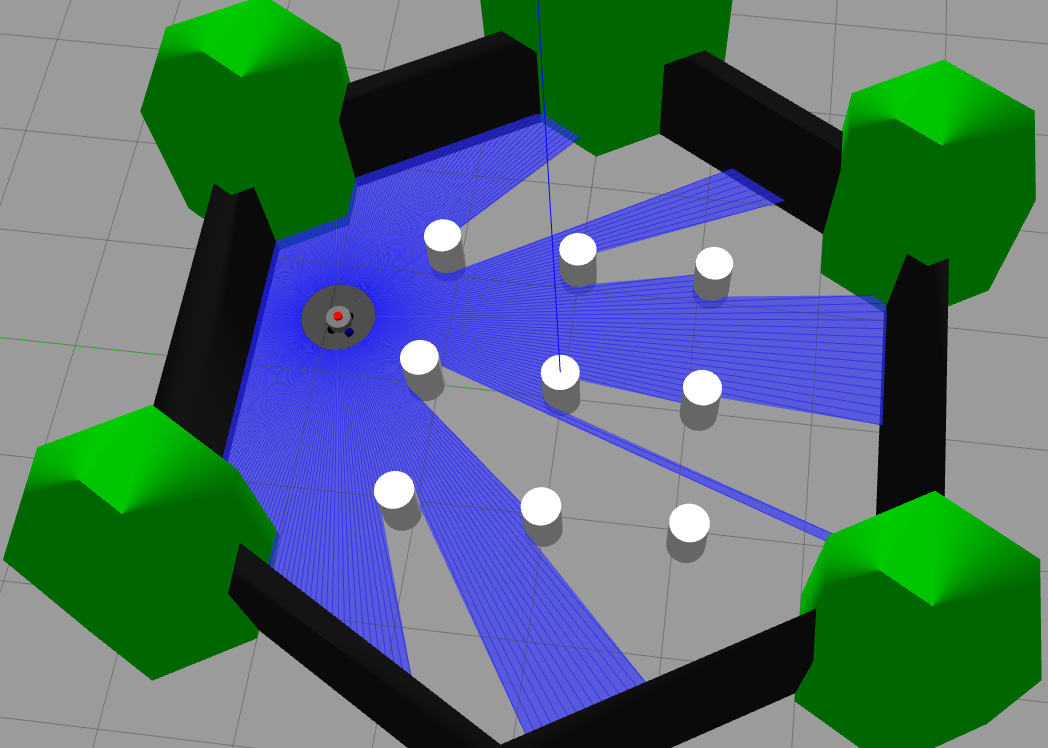
\includegraphics[width=\columnwidth]{images/simulation_map.png}
    \caption{Simulation test environment, also showing the simulated robot.}
    \label{fig:simulation_map}
\end{figure}

%------------------------------------------------------------------------------------------
% Real world

\subsection{Real-world}
\label{subsection:real_world}

% Integration (how our system works)
Four ROS2 nodes were running on the robot (Raspberry Pi), these are the robot-state-publisher, rplidar, mpu6050 and ros2-control. The robot-state-publisher publishes the joint state values for the wheels, the mpu6050 publishes the IMU sensor values and rplidar publishes the LIDAR sensor values.
Finally, the ros2-control node takes the desired input velocity and communicates this through a hardware interface to the Arduino Nano which in turn controls the wheels.
The SLAM Toolbox, Nav2 and EKF filtering nodes were running on an external PC and works the same as in the simulation, issuing of waypoints also works the same as in simulation (see Method\:\ref{subsection:simulation}).

% Test environment (features)
The robot was deployed in an apartment which served as the real-world test environment and can be seen in Fig.\:\ref{fig:real_world_map}. The test environment thus consisted of a static indoor environment which had constant lighting and was open. 
% Test scenario
The real-world testing scenario involved a mapping session where the robot mapped the entire testing environment.
% Evaluation metrics
The real-world deployment of the system was evaluated in terms of the following metrics:
\begin{itemize}
    \item SLAM map compared to ground truth map
    \item Number of collisions
    \item Processing time per sensor update (ms)
\end{itemize}

\begin{figure}
    \centering
    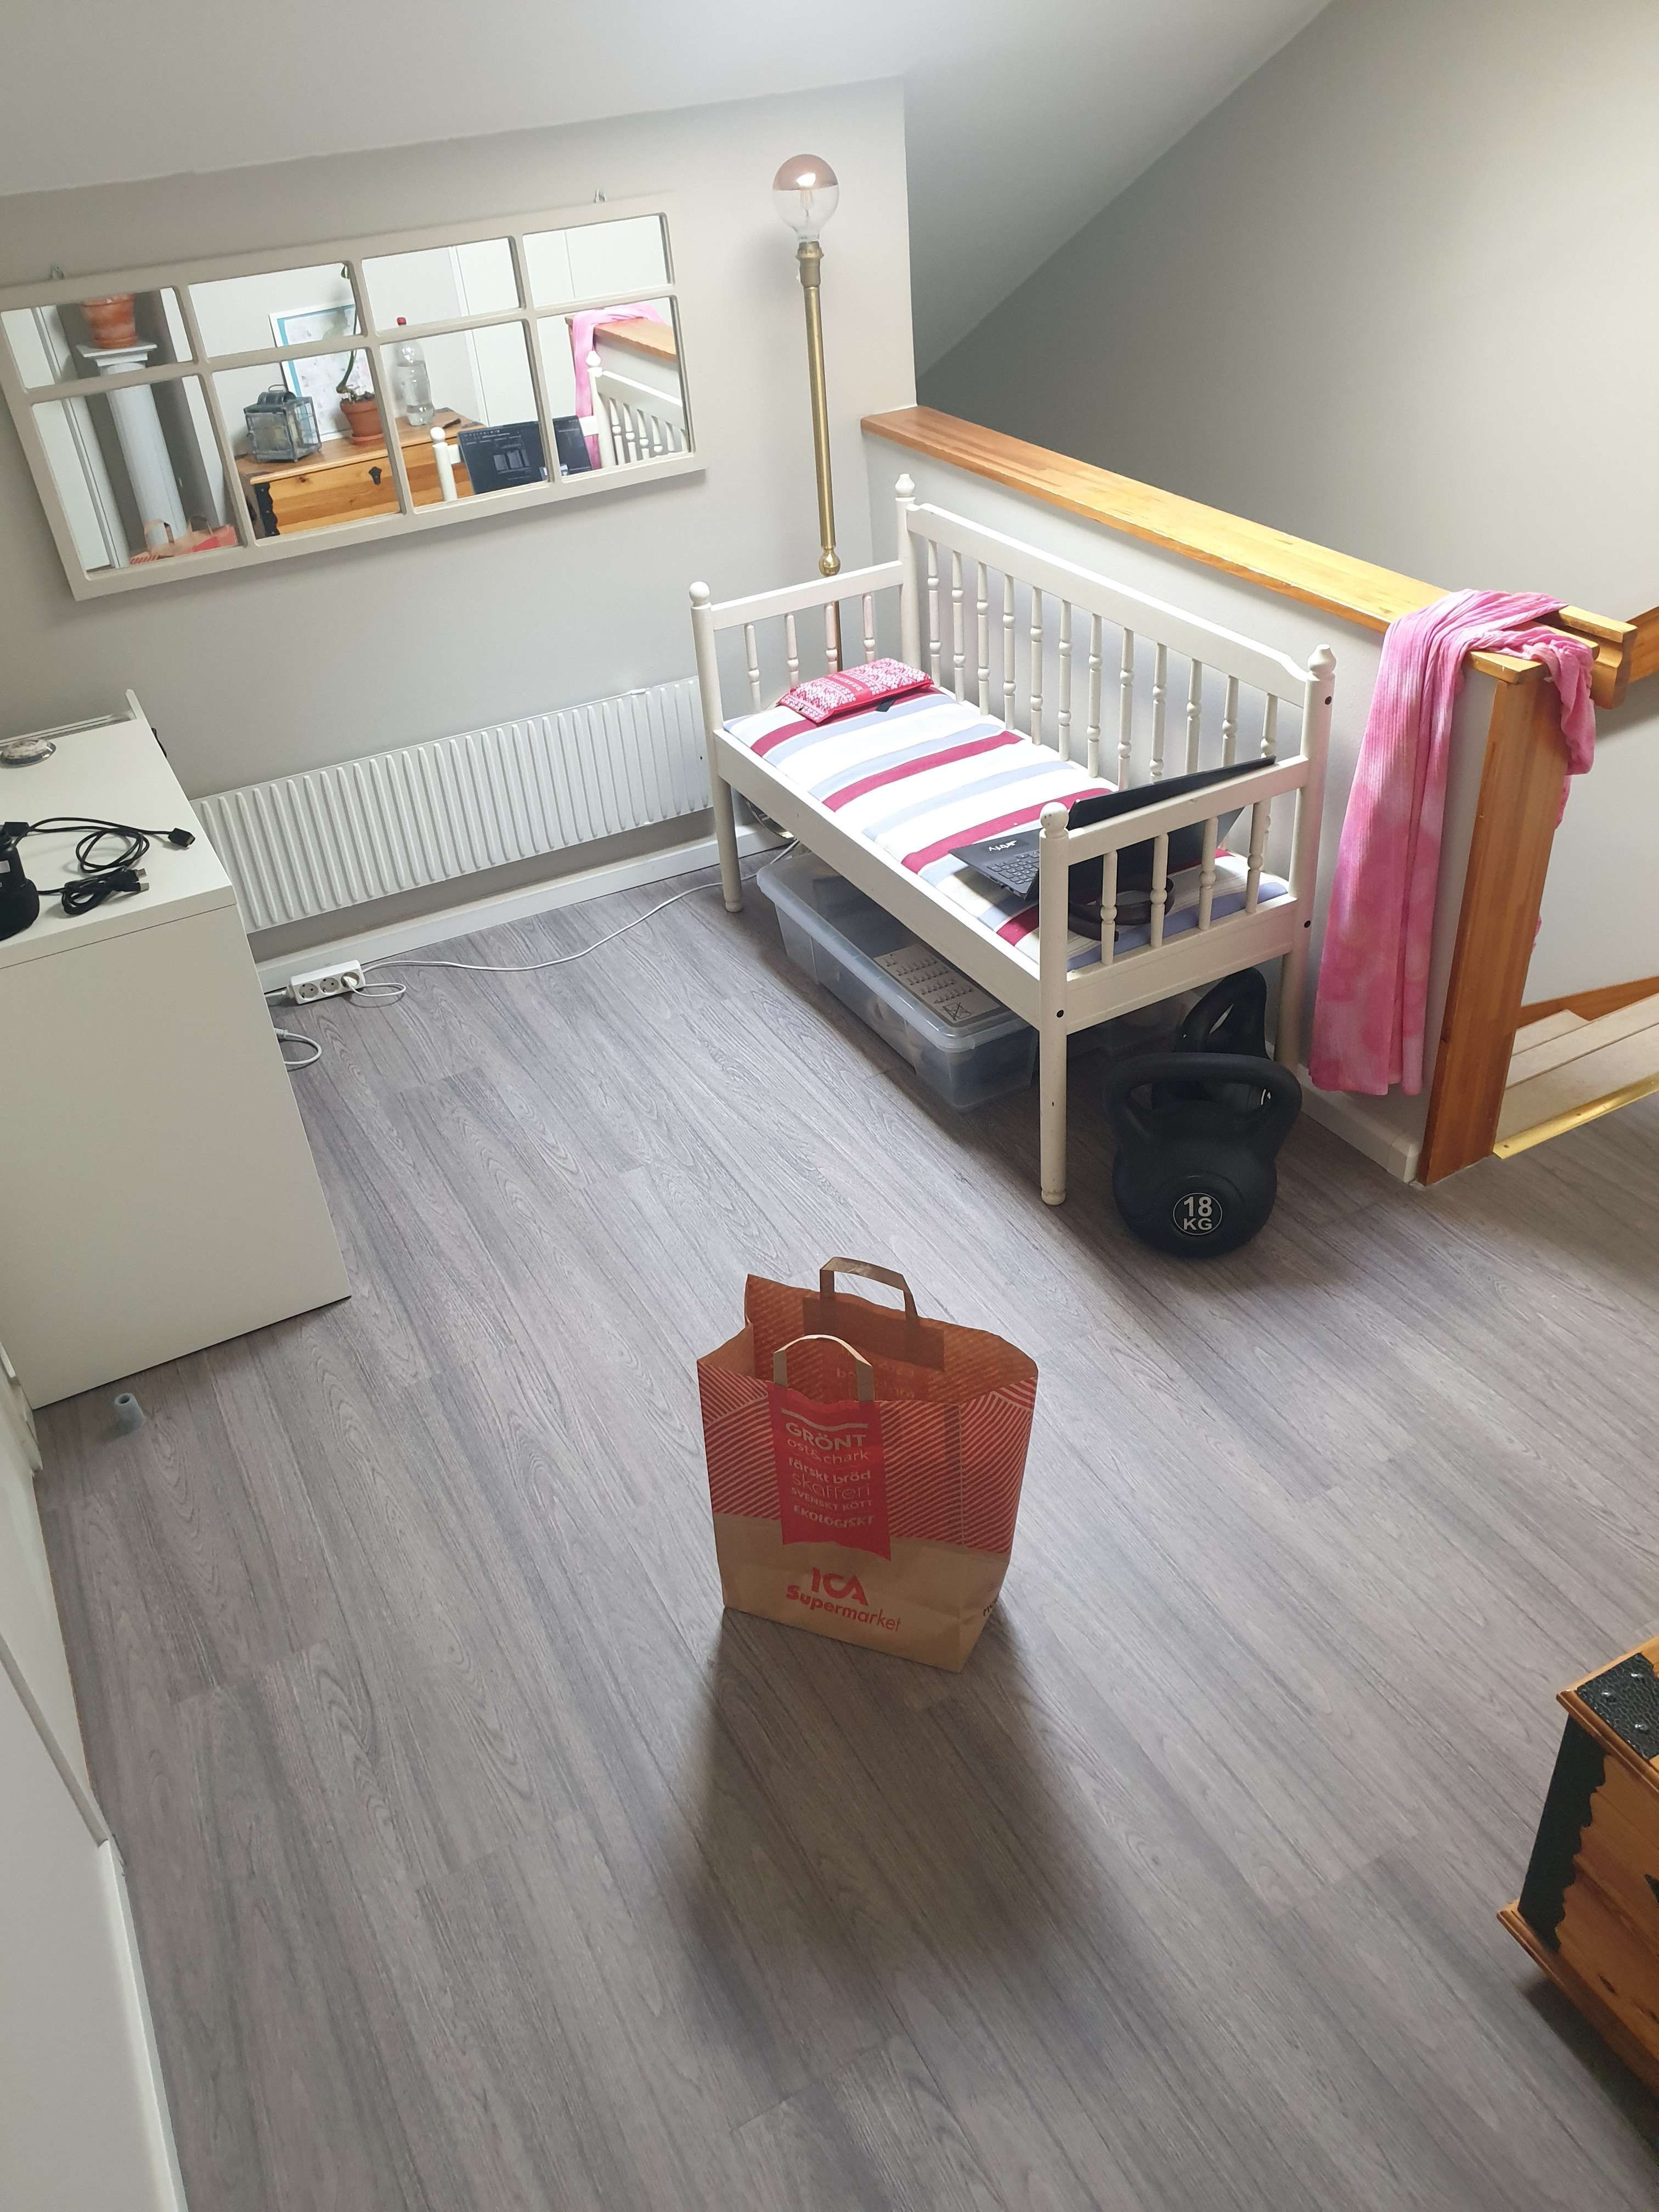
\includegraphics[width=\columnwidth]{images/real_world_map.jpg}
    \caption{Real-world test environment.}
    \label{fig:real_world_map}
\end{figure}

%------------------------------------------------------------------------------------------


%------------------------------------------------------------------------------------------
\begin{comment}
    Italicize symbols ($T$ might refer to temperature, but T is the unit tesla).

    Refer to ``\eqref{eq},'' not ``Eq. \eqref{eq}''
    
    It is good practice to explain the significance of the figure in the caption.
    
    Figure axis labels are often a source of confusion. Use words rather than symbols. As an example, write the quantity ``Magnetization,'' or ``Magnetization M,'' not just ``M.'' Put units in parentheses. Do not label axes only with units. As in Fig. 1, for example, write ``Magnetization (A/m)'' or ``Magnetization (A$\cdot$m$^{-1}$),'' not just ``A/m.'' Do not label axes with a ratio of quantities and units. For example, write ``Temperature (K),'' not ``Temperature/K.''
    
    When referencing your figures and tables within your paper, use the abbreviation ``Fig.'' even at the beginning of a sentence. Do not abbreviate ``Table.'' Tables should be numbered with Roman Numerals.
      
    In this section, the method used to find an answer to the research questions should be presented.
    
    If this report presents results from a literature search, this means providing sufficient information for allowing someone else to repeat the literature search and compare the results. I.e., a search using the phrases a, b, and c, was made in database x, y and z on the date Month Date, Year (e.g., July 31st, 2021). The search resulted in x hits. Then, information on how you chose which works to include in this report should be provided. The references should be used for answering your research questions.
    
    If the work reports on an experiment, this part should provide information about the experimental setup, how the experiment was conducted, how data was collected and analyzed etc. Motivate methodological choices through references. Also an experiment should be presented with sufficient detail such that it can be repeated by someone else.
\end{comment}
%------------------------------------------------------------------------------------------